

%\documentclass{acm_proc_article-sp}
%\documentclass{sig-alternate}
\documentclass[conference]{IEEEtran}
\usepackage{multirow}
\usepackage{fancyheadings}
\usepackage{algorithmic}
\usepackage{amssymb}
\usepackage{amsmath}
\usepackage{xspace}
\usepackage{pslatex}
\usepackage{microtype}
\usepackage{subfigure}
\usepackage{indentfirst}
\usepackage{listings, algorithm, algorithmic, graphicx, listing}
\usepackage{relsize}

%\usepackage{todonotes}
\usepackage{times}
\usepackage{graphicx}
\usepackage{epsf}
\usepackage{verbatim}
%\usepackage{psfig}
\usepackage{cite}
\usepackage{url}
\usepackage{color}
\usepackage{alltt}

\newcommand{\StateProjection}{static analysis}
\newcommand{\CurAspectJSubjectCount}{12}

\newcommand{\Add}{\CodeIn{add}}
\newcommand{\AVTree}{\CodeIn{AVTree}}
\newcommand{\Assignment}[3]{$\langle$ \Object{#1}, \Object{#2}, \Object{#3} $\rangle$}
\newcommand{\BinaryTreeRemove}{\CodeIn{BinaryTree\_remove}}
\newcommand{\BinaryTree}{\CodeIn{BinaryTree}}
\newcommand{\Caption}{\caption}
\newcommand{\Char}[1]{`#1'}
\newcommand{\CheckRep}{\CodeIn{checkRep}}
\newcommand{\ClassC}{\CodeIn{C}}
\newcommand{\CodeIn}[1]{{\small\texttt{#1}}}
\newcommand{\CodeOutSize}{\scriptsize}
\newcommand{\Comment}[1]{}
\newcommand{\Ensures}{\CodeIn{ensures}}
\newcommand{\ExtractMax}{\CodeIn{extractMax}}
\newcommand{\FAL}{field-ordering}
\newcommand{\FALs}{field-orderings}
\newcommand{\Fact}{observation}
\newcommand{\Get}{\CodeIn{get}}
\newcommand{\HashSet}{\CodeIn{HashSet}}
\newcommand{\HeapArray}{\CodeIn{HeapArray}}
\newcommand{\Intro}[1]{\emph{#1}}
\newcommand{\Invariant}{\CodeIn{invariant}}
\newcommand{\JUC}{\CodeIn{java.\-util.\-Collections}}
\newcommand{\JUS}{\CodeIn{java.\-util.\-Set}}
\newcommand{\JUTM}{\CodeIn{java.\-util.\-TreeMap}}
\newcommand{\JUTS}{\CodeIn{java.\-util.\-TreeSet}}
\newcommand{\JUV}{\CodeIn{java.\-util.\-Vector}}
\newcommand{\JMLPlusJUnit}{JML+JUnit}
\newcommand{\Korat}{Korat}
\newcommand{\Left}{\CodeIn{left}}
\newcommand{\Lookup}{\CodeIn{lookup}}
\newcommand{\MethM}{\CodeIn{m}}
\newcommand{\Node}[1]{\CodeIn{N}$_#1$}
\newcommand{\Null}{\CodeIn{null}}
\newcommand{\Object}[1]{\CodeIn{o}\ensuremath{_#1}}
\newcommand{\PostM}{\MethM$_{post}$}
\newcommand{\PreM}{\MethM$_{pre}$}
\newcommand{\Put}{\CodeIn{put}}
\newcommand{\Remove}{\CodeIn{remove}}
\newcommand{\RepOk}{\CodeIn{repOk}}
\newcommand{\Requires}{\CodeIn{requires}}
\newcommand{\Reverse}{\CodeIn{reverse}}
\newcommand{\Right}{\CodeIn{right}}
\newcommand{\Root}{\CodeIn{root}}
\newcommand{\Set}{\CodeIn{set}}
\newcommand{\State}[1]{2^{#1}}
\newcommand{\TestEra}{TestEra}
\newcommand{\TreeMap}{\CodeIn{TreeMap}}

\newenvironment{CodeOut}{\begin{scriptsize}}{\end{scriptsize}}
\newenvironment{SmallOut}{\begin{small}}{\end{small}}

\newcommand{\pairwiseEquals}{PairwiseEquals}
\newcommand{\monitorEquals}{MonitorEquals}
%\newcommand{\monitorWField}{WholeStateW}
\newcommand{\traverseField}{WholeState}
\newcommand{\monitorSMSeq}{ModifyingSeq}
\newcommand{\monitorSeq}{WholeSeq}

\newcommand{\IntStack}{\CodeIn{IntStack}}
\newcommand{\UBStack}{\CodeIn{UBStack}}
\newcommand{\BSet}{\CodeIn{BSet}}
\newcommand{\BBag}{\CodeIn{BBag}}
\newcommand{\ShoppingCart}{\CodeIn{ShoppingCart}}
\newcommand{\BankAccount}{\CodeIn{BankAccount}}
\newcommand{\BinarySearchTree}{\CodeIn{BinarySearchTree}}
\newcommand{\LinkedList}{\CodeIn{LinkedList}}

\newcommand{\Book}{\CodeIn{Book}}
\newcommand{\Library}{\CodeIn{Library}}

\newcommand{\Jtest}{Jtest}
\newcommand{\JCrasher}{JCrasher}
\newcommand{\Daikon}{Daikon}
\newcommand{\JUnit}{JUnit}

\newcommand{\trie}{trie}

\newcommand{\Perl}{Perl}


\newcommand{\SubjectCount}{11}
\newcommand{\DSSubjectCount}{two}

\newcommand{\Equals}{\CodeIn{equals}}
\newcommand{\Pairwise}{PairwiseEquals}
\newcommand{\Subgraph}{MonitorEquals}
\newcommand{\Concrete}{WholeState}
\newcommand{\ModSeq}{ModifyingSeq}
\newcommand{\Seq}{WholeSeq}
\newcommand{\Aeq}{equality}

\newcommand{\Meaning}[1]{\ensuremath{[\![}#1\ensuremath{]\!]}}
\newcommand{\Pair}[2]{\ensuremath{\langle #1, #2 \rangle}}
\newcommand{\Triple}[3]{\ensuremath{\langle #1, #2, #3 \rangle}}
\newcommand{\SetSuch}[2]{\ensuremath{\{ #1 | #2 \}}}
%\Comment{
%\newtheorem{definition}{Definition}
%\newtheorem{theorem}[definition]{Theorem}
%}
\newcommand{\Equiv}[2]{\ensuremath{#1 \EquivSTRel{} #2}}
\newcommand{\EquivME}{\Equiv}
\newcommand{\EquivST}{\Equiv}
\newcommand{\EquivSTRel}{\ensuremath{\cong}}
\newcommand{\Redundant}[2]{\ensuremath{#1 \lhd #2}}
\newcommand{\VB}{\ensuremath{\mid}}
\newcommand{\MES}{method-entry state}

\newcommand{\Small}[1]{{\small{#1}}}

\newcommand{\CenterCell}[1]{\multicolumn{1}{c|}{#1}}
\newcommand{\Fix}[1]{{\large\textbf{FIX}}#1{\large\textbf{FIX}}}

\newcommand{\CodeInS}[1]{{\scriptsize\texttt{#1}}}
\newcommand{\CodeInFN}[1]{{\footnotesize\texttt{#1}}}
\newcommand{\CodeOutFN}{\footnotesize}

\newcommand{\SmallSpace}{\vspace*{-1.4ex}}
\newcommand{\Item}{\SmallSpace\item}
\newenvironment{Itemize}{\begin{itemize}}{\end{itemize}\SmallSpace}
\newenvironment{Enumerate}{\begin{enumerate}}{\end{enumerate}\SmallSpace}

\newtheorem{definition}{Definition}
\newtheorem{theorem}[definition]{Theorem}

%\newcommand{\Item}{\vspace*{-0.5ex}\item\vspace*{-0.5ex}}
%\newenvironment{Itemize}{\begin{itemize}\vspace*{-1ex}}{\end{itemize}\vspace*{-1ex}}
%\newenvironment{Enumerate}{\begin{enumerate}\vspace*{-1ex}}{\end{enumerate}\vspace*{-1ex}}
\newenvironment{Definition}{\begin{definition}\vspace*{-1.5ex}}{\end{definition}\vspace*{-1.5ex}}

% Local Variables:
% mode:latex
% End:


% % Add line between figure and text
 \makeatletter
 \def\topfigrule{\kern3\p@ \hrule \kern -3.4\p@} % the \hrule is .4pt high
 \def\botfigrule{\kern-3\p@ \hrule \kern 2.6\p@} % the \hrule is .4pt high
 \def\dblfigrule{\kern3\p@ \hrule \kern -3.4\p@} % the \hrule is .4pt high
 \makeatother

 % If there is a line, you can get away with reducing the separation between
 % figures and text.  Don't do this without the line, though.
 \addtolength{\textfloatsep}{-.5\textfloatsep}
 \addtolength{\dbltextfloatsep}{-.5\dbltextfloatsep}
 \addtolength{\floatsep}{-.5\floatsep}
 \addtolength{\dblfloatsep}{-.5\dblfloatsep}

% Left and right curly braces in tt font
\newcommand{\ttlcb}{\texttt{\char "7B}}
\newcommand{\ttrcb}{\texttt{\char "7D}}

\newcommand{\totaloc}{99458 }
\newcommand{\subnum}{10 }
\newcommand{\warnings}{22 }
\newcommand{\bugs}{12 }
\newcommand{\newbugs}{7 }
\newcommand{\falses}{10 }
\newcommand{\annotationnum}{7 }
\newcommand{\filternum}{11 }

% \newcommand{\smallstep}{\vspace{-2mm}}
% \newcommand{\tinystep}{\vspace{-1mm}}
\newcommand{\smallstep}{\relax}
\newcommand{\tinystep}{\relax}


\newenvironment{myindentpar}[1]%
{\begin{list}{}%
         {\setlength{\leftmargin}{#1}}%
         \item[]%
}
{\end{list}}


% Reduce indentation in lists.
%\setlength{\leftmargini}{.5\leftmargini}

%% Bring items closer together in list environments
%% This doesn't work with an optional argument to the list environment.
% Prevent infinite loops
\let\Itemize =\itemize    
\let\Enumerate =\enumerate
\let\Description =\description
% Zero the vertical spacing parameters
\def\Nospacing{\itemsep=0pt\topsep=0pt\partopsep=0pt\parskip=0pt\parsep=0pt}
% Redefine the environments in terms of the original values
\renewenvironment{itemize}{\Itemize\Nospacing}{\endlist}
\renewenvironment{enumerate}{\Enumerate\Nospacing}{\endlist}
\renewenvironment{description}{\Description\Nospacing}{\endlist}

%\newcommand{\todo}[1]{{TODO #1}}
\newcommand{\todo}[1]{{\color{red}\bfseries [[{#1}]]}}
\newcommand{\sai}[1]{{\color{blue}\todo{for Sai: #1}}}
\newcommand{\yuyin}[1]{{\color{red}\todo{for Yuyin: #1}}}

\newcommand{\ourtool}{SQLSynthesizer\xspace}

\newcommand{\exnum}{XXX\xspace}
\newcommand{\solexnum}{XXX\xspace}

\newcommand{\pnum}{XXX\xspace}
\newcommand{\solpnum}{XXX\xspace}

\begin{document}

\title{Automatically Synthesizing SQL Queries from \\Input-Output Examples}



\author{\IEEEauthorblockN{Sai Zhang\quad Yuyin Sun}
\IEEEauthorblockA{Computer Science \& Engineering\\
University of Washington, USA\\
\{szhang, sunyuyin\}@cs.washington.edu}}


\maketitle

\begin{abstract}

In the age of big data, a large number of computer end-users, such as
research scientists and business analysts, need to frequently query
a database, yet lack the programming knowledge to do such tasks smoothly.
In this paper, we present a \textit{programming by example} technique
that permits end-users to automate such querying tasks.
Our technique takes from users an input and output example of how the
database should be queried, and synthesizes a SQL query that
reproduces the example output from the example input. Later, when the synthesized
SQL query is applied to another, potentially larger, database with a
similar schema as the example input, the synthesized SQL query produces
a corresponding result that is similar to the example output. Our technique
has several notable features: it only needs small input-output examples
to infer a desirable SQL query, it is fully automated and does not require
users to provide annotations/hints of any form, and it can rank multiple
possible solutions to provide to users the most likely result.


Our technique has been implemented as an open-source programming
tool. In our preliminary evaluation, our prototype tool has synthesized correct
answers for 5 out of 6 SQL exercises from a classic database textbook,
and has been used to solve 5 non-trivial problems raised by real-world
users from popular online forums, including ones that receive no human replies.

%This opens up an amazing
%set of possibilities in the context of making classroom teaching
%interactive


\end{abstract}


\section{Introduction}
\label{sec:introduction}

\vspace{-1mm}

The big data revolution has resulted in digitization of massive amounts
of data. There is a growing population
of non-expert database end-users, who need to perform
analysis on their databases, but have limited programming knowledge.

%A key challenge faced by many
%enterprise and computer end-users nowadays is the management
%of their increasingly large and complex databases.
%, which can contain
%hundreds and even thousands of tables. 


%but they often need to
%query databases to obtain relevant data to support their business decisions.


%\subsection{End-users' Difficulties in Writing SQL Queries}
%\vspace{1mm}
%\noindent \textbf{\textit{Motivation.}}
Although relational database management systems (RDBMS) and the
de facto standard query language (SQL) are perfectly adequate for most end-users'
needs, 
the costs associated with use of database and SQL are non-trivial~\cite{Howe:2011}. 
The problem is exacerbated by the fact that end-users
have diverse backgrounds and include
business analysts, commodity traders, 
finance professionals, and marketing managers. 
They are not professional programmers.
They need to retrieve information from their
databases and use the information to support their business decisions.
Although most end-users can clearly describe \textit{what} the task is, they
are often stuck with the process of \textit{how} to
write a correct database query (i.e., a SQL query).
% even after
%receiving step-by-step, detailed,
%and syntactically correct instructions.
Thus, non-expert end-users often need to
seek information from online help forums or
SQL experts. This process can be laborious and frustrating.
Non-expert end-users need
a tool that can be used to ``describe''
their needs and ``connect'' their intentions to executable
SQL queries.

%simply can not get the SQL query correct,
%either due to the syntax complexity of the SQL language itself,
%or the structure complexity of the databases.
%To write a correct SQL query, end-users often need to
%seek information from online help forums, or ask
%SQL experts. This process can be repetative, laborious, and frustrating.

%However, such practice is inefficient and time-consuming.
%Non-professional end-users 


%\todo{move the following sentence to somewhere esle}

%Similarly, other end-users
%such as business analysts who query databases frequently often
%do not have significant SQL expertise.

%To learn how to query a RDBMS, most end-users often refer
%to a textbook or online resources to first get familiar with
%the basic idioms of the SQL language. Then, they may
%try to write some experimental queries, execute them
%on a sample database to observe the output, and
%subsequently revise the queries (if the output is not desirable).

%The above process may
%predicates in the \CodeIn{where} clause,
%tables in the \CodeIn{from} clause, or columns in the \CodeIn{select} clauses.



%\subsection{Existing Solutions}

\vspace{1mm}
\noindent \textbf{\textit{Existing solutions.}}
\textit{Graphical User Interfaces} (GUIs) and \textit{programming languages}
are two state-of-the-art approaches to help end-users perform
database queries. However, both approaches have limitations.

Many RDBMSes come with a well-designed GUI with lots of features.
However, 
%as a database management system often comes with tons
%of features, end-users struggle to find the correct feature or
%succession of commands to use from a maze of features to accomplish
%their tasks.
a GUI is often fixed, and does not permit users to personalize
a database's functionality for their query tasks. On the other hand,
as a GUI supports more and more customization features, users
may struggle to discover those features, which can significantly
degrade its usability. 

Programming languages, such as SQL and
other domain-specific query languages (e.g., Java with JDBC), 
are a fully expressive medium  for
communicating a user's intention to a database. However, 
general programming languages have never been easy for
end-users who are not professional programmers.  Learning
a practical programming language (even a simplified domain-specific language, such as MDX~\cite{mdx}) often requires a substantial amount
of time and energy that a typical end-user would not prefer,
and should not be expected, to invest. 



%\subsection{Synthesizing SQL Queries from Input-Output Examples}

%After carefully studying how end-users were describing their
%encountered SQL query problems on online help forums, we observed that
%one of the most common ways for end-users to
%express their intents is using input-output examples. 

\vspace{1mm}
\noindent \textbf{\textit{Our solution: synthesizing SQL queries from input-output examples.}}
This paper presents a technique (and its tool
implementation, called \ourtool) to automatically
synthesize SQL queries\footnote{
All queries mentioned in this paper refer to SQL queries
that retrieve data from a database but
do not update its content.}
from input-output examples.
Although input-output examples may lead to
underspecification, writing them, as opposed to writing
declarative specifications or imperative code
of any form, is one of the easiest ways
for end-users to describe \textit{what} the task is.
%\ourtool takes example input
%table(s) and output table from the end-users, and then automatically
%infers a SQL query (or multiple queries, if exist) that queries
%against the input tables and returns the output example.
If the synthesized SQL query is applied
to the example input, then it produces the example output; and if the
synthesized SQL query is applied to other
similar input (potentially much larger tables),
then it produces a corresponding output.


%\ourtool uses such input-output examples
%as a natural interface to "understand" an end-user's intention
%and provide corresponding assistance.

%Compared with other alternatives (such as, writting
%a declarative specification) to specify a user's intention,
%input-output examples, although may lead to underspecification,
%serve as a more straightforward way  is and a natural interface that a tool can provide assistance.

\ourtool is designed to be used by non-expert database
end-users when they do not know how
to write a correct SQL query. 
End-users can use \ourtool to obtain a SQL query to transform
multiple, huge database tables by constructing small, representative
input and output example tables. 
We also envision \ourtool to be useful in an online education
setting (i.e., an online database course). 
Education initiatives such as Udacity~\cite{udacity} and Coursera~\cite{coursera}
 are teaming up with experts to provide
high-quality online courses to thousands of students worldwide.
One challenge, which is not present in a traditional classroom
setting, is to provide answers to questions raised by a large
number of students. A tool, like \ourtool,
that has the potential of answering SQL query related questions
would be useful.
%preferrable in \todo{teaching a database course.}
%helping end-users writing a wide range of SQL queries.


Inferring SQL queries from examples is challenging,
primarily for two reasons. First, the standard SQL
language is inherently complex; a SQL query can consist
of many parts, such as joins, aggregates,
the \CodeIn{GROUP BY} clause, and the \CodeIn{ORDER BY} clause.
Searching for a SQL query
to satisfy a given example input and output pair,
as proved by Sarma et al.~\cite{DasSarma:2010},
is a PSPACE-hard problem. Thus,
a brute-force approach such as exhaustively
enumerating all
syntactically-valid SQL queries and then
filtering away those do not satisfy the examples
becomes intractable in practice. 
Second, a SQL query has a rich set of operations: it
needs to be evaluated on \textit{multiple} input tables;
it needs to perform data grouping, selection, and ordering
operations; and it needs to project data on certain columns to
form the output.
All such operations must be inferred properly and efficiently.% This requires \todo{new challenges}
%unlike a spreadsheet macro  that
%re-shapes one input table to one output table~\cite{Harris:2011},


To address these challenges and make example-based
SQL query synthesis feasible in practice,
\ourtool focuses on a widely-used SQL subset (Section~\ref{sec:langsubset})
and uses three steps to link a user's intention to
a SQL query (Section~\ref{sec:approach}):



\begin{itemize}
\vspace{-1mm}
\item \textbf{Skeleton Creation.} \ourtool scans the
given input-output examples and heuristically
determines table joins and projection columns in
the result query. Then, it creates an
incomplete SQL query (called a query skeleton) to
capture the basic structure of the result query.

\item \textbf{Query Completion.} \ourtool
uses a machine learning algorithm to infer a set of accurate
and expressive rules, which transforms the input
example into the output example. Then, it
searches for other missing parts in a query skeleton,
%possible aggregates and columns in
%the \CodeIn{ORDER BY} clause; 
and builds a list of candidate queries. 


\item \textbf{Candidate Ranking.} If multiple SQL
queries satisfy the given input-output examples,
\ourtool employs the Occam's razor principle to
rank simpler queries higher in the output.
\end{itemize}

Compared to previous approaches~\cite{Zloof:1975,
Tran:2009, DasSarma:2010, abs-1208-2013}, \ourtool has two notable features:

\begin{itemize}
\item \textbf{It is fully automated.} Besides
an example input and output pair,
\ourtool does not require users to provide
annotations or hints of any form. 
This distinguishes our work from competing techniques such as
specification-based query inference~\cite{Zloof:1975} and
query synthesis from imperative code~\cite{abs-1208-2013}.

\item \textbf{It supports a wide range of SQL queries.}
Similar approaches in the literature support
a small subset of the SQL language; and most of them
can only infer simple select-from-where
queries on a single table~\cite{Zloof:1975, Tran:2009, DasSarma:2010, abs-1208-2013}. By contrast, 
\ourtool significantly enriches the supported SQL subset.
Besides supporting standard select-from-where
queries, \ourtool also supports many advanced
SQL features, such as table joins,
aggregates (e.g., \CodeIn{MAX}, \CodeIn{MIN}, \CodeIn{SUM},
and \CodeIn{COUNT}), the \CodeIn{GROUP BY} clause,
the \CodeIn{ORDER BY} clause, and the \CodeIn{HAVING} clause.
%\item \textbf{It requires small input-output examples.}
\end{itemize}


%is usually the correct one. 

%Besides
%selecting a smaller one, we could also compute the likelihood
%of each query being correct based on some statistics, and then
%pick the most likely one.


%\subsection{Evaluation}

\vspace{1mm}
\noindent \textbf{\textit{Evaluation}}.
We evaluated \ourtool's generality and accuracy
in two aspects. First, we used \ourtool to solve
\exnum SQL exercises from a classic database textbook~\cite{cowbook}. 
We used textbook exercises because they
are often designed to cover a wide range of SQL features.
Some exercises are even designed on purpose
to be challenging and to cover some less realistic,
corner cases in using SQL.
%the most important
%SQL features that an instructor wishes students to master,
Second, we evaluated \ourtool on \pnum SQL query related
questions collected from popular online help forums, and tested whether
\ourtool can synthesize correct SQL queries for them.

As a result, \ourtool successfully synthesized queries
for \solexnum out of \exnum textbook exercises and
all \pnum forum problems, within a very small amount of time
(\avgsucctime seconds per exercise or problem, on average).
\ourtool's accuracy and speed make it an attractive
tool for end-users to use.% write SQL queries.

%\subsection{Contributions}

\vspace{1mm}
\noindent\textbf{\textit{Contributions.}}
This paper makes the following contributions:

\begin{itemize}
%\item \textbf{Problem.} To the best of our knowledge, we are the first
%to address the SQL query synthesis problem from examples across multiple
%tables.
%An approach to automatically synthesizing SQL
%queries from input-output examples (Section~\ref{sec:approach}).

\item \textbf{Technique.} We present a technique that automatically
synthesizes SQL queries from input-output examples
(Section~\ref{sec:approach}).

\item \textbf{Implementation.} We implemented our technique in a
tool, called \ourtool (Section~\ref{sec:implementation}). It is
available at: \url{http://sqlsynthesizer.googlecode.com}.

\item \textbf{Evaluation.} We applied \ourtool
to \exnum textbook exercises and \pnum 
forum questions.
The experimental results show that \ourtool is
useful in synthesizing SQL queries with
small examples (Section~\ref{sec:evaluation}).
\end{itemize}



\begin{figure*}[t]
  \centering
  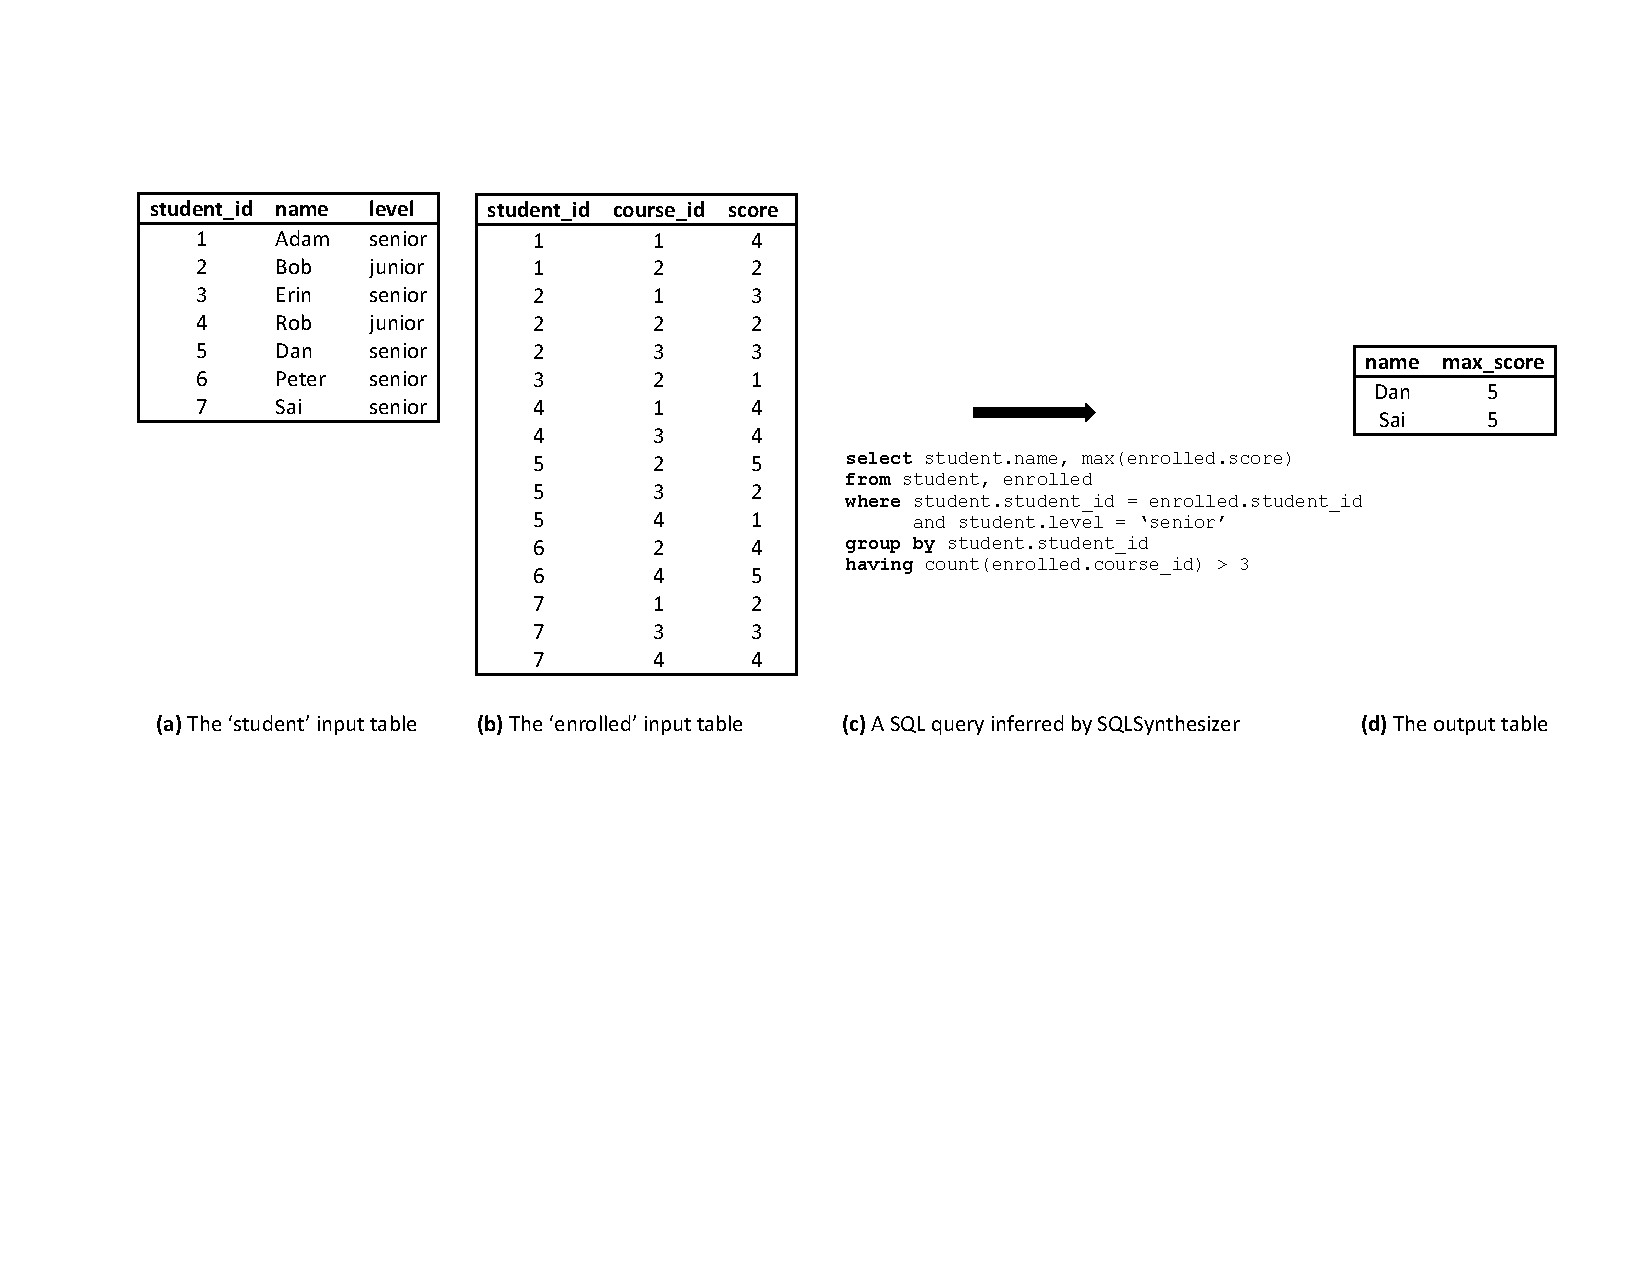
\includegraphics[scale=0.75]{motivating}
  \vspace*{-4.0ex}\caption {{\label{fig:motivating}
  Illustration of how to use \ourtool to solve the problem in Section~\ref{sec:example}. Users provide \ourtool with
  two input tables (shown in (a)) and an output table (shown in (c)).
  \ourtool automatically synthesizes a SQL query (shown in (b)) that
  transforms the two input tables into the output table.
}}
\end{figure*}

\section{Illustrating Example}
\label{sec:example}

We use an example, described below, to illustrate the use
of \ourtool. The example is taken from a classic
database textbook~\cite{cowbook} (Chapter 5, Exercise 1)
and has been simplified for illustration purpose\footnote{
This exercise defines 2 tables: \CodeIn{student}
and \CodeIn{enrolled}. The \CodeIn{student} table
contains three columns: \CodeIn{student\_id}, \CodeIn{name},
and \CodeIn{level}. Table \CodeIn{enrolled} also contains
three columns: \CodeIn{student\_id}, \CodeIn{course\_id},
and \CodeIn{score}.
}.

\begin{quote}
\textit{Find the name and the maximum course score of each senior student
enrolled in more than 2 courses.}
\end{quote}

Despite the simplicity of the problem description,
writing a correct SQL query  can be non-trivial for a typical
end-user. An end-user must carefully choose the
right SQL features and use them correctly
to fulfill the described task.
%Although most users can clearly understand the
%question, they must choose the right SQL
%features and use them correctly.

As an alternative, users can use \ourtool to obtain
the desirable query.
%As illustrated in Figure~\ref{fig:motivating},
To use \ourtool, an end-user only needs to provide it with
some small, representative example input and output tables
(Figures~\ref{fig:motivating}(a) and~\ref{fig:motivating}(c)).
Then, \ourtool works in a fully-automatic, push-button
way to infer a SQL query that satisfies the given
example input and output.

 %illustrate in Figure~\ref{fig:motivating}, an alternative
%approach to write this query is to provide \ourtool
%with some representative input-output examples; and
%let \ourtool automatically automatically infer the query.

The SQL query, shown in Figure~\ref{fig:motivating}(b),
first joins two tables on the common \CodeIn{student\_id} column,
and then groups the joined results by the \CodeIn{student\_id}
column. Further, the query selects all senior
students (using a query condition in the \CodeIn{WHERE}
clause) who are enrolled in more than 2 courses
(using a condition in the \CodeIn{HAVING} clause).
Finally, the query projects the result on the
\CodeIn{student.name} column and uses the \CodeIn{MAX} aggregate
to compute the maximum course score.

%the \CodeIn{student} with \CodeIn{enrolled} tables,
%then group bys the joined table by the \CodeIn{student\_id}
%column, and selects students enrolled in more
%than 2 courses (using the \CodeIn{having} statement).
%After that, the query further selects students
%whose level is \CodeIn{senior} and uses the \CodeIn{max}
%aggregator function to compute the maximum course score.
%\todo{the above needs polish}









\begin{figure}[t]
  \centering
  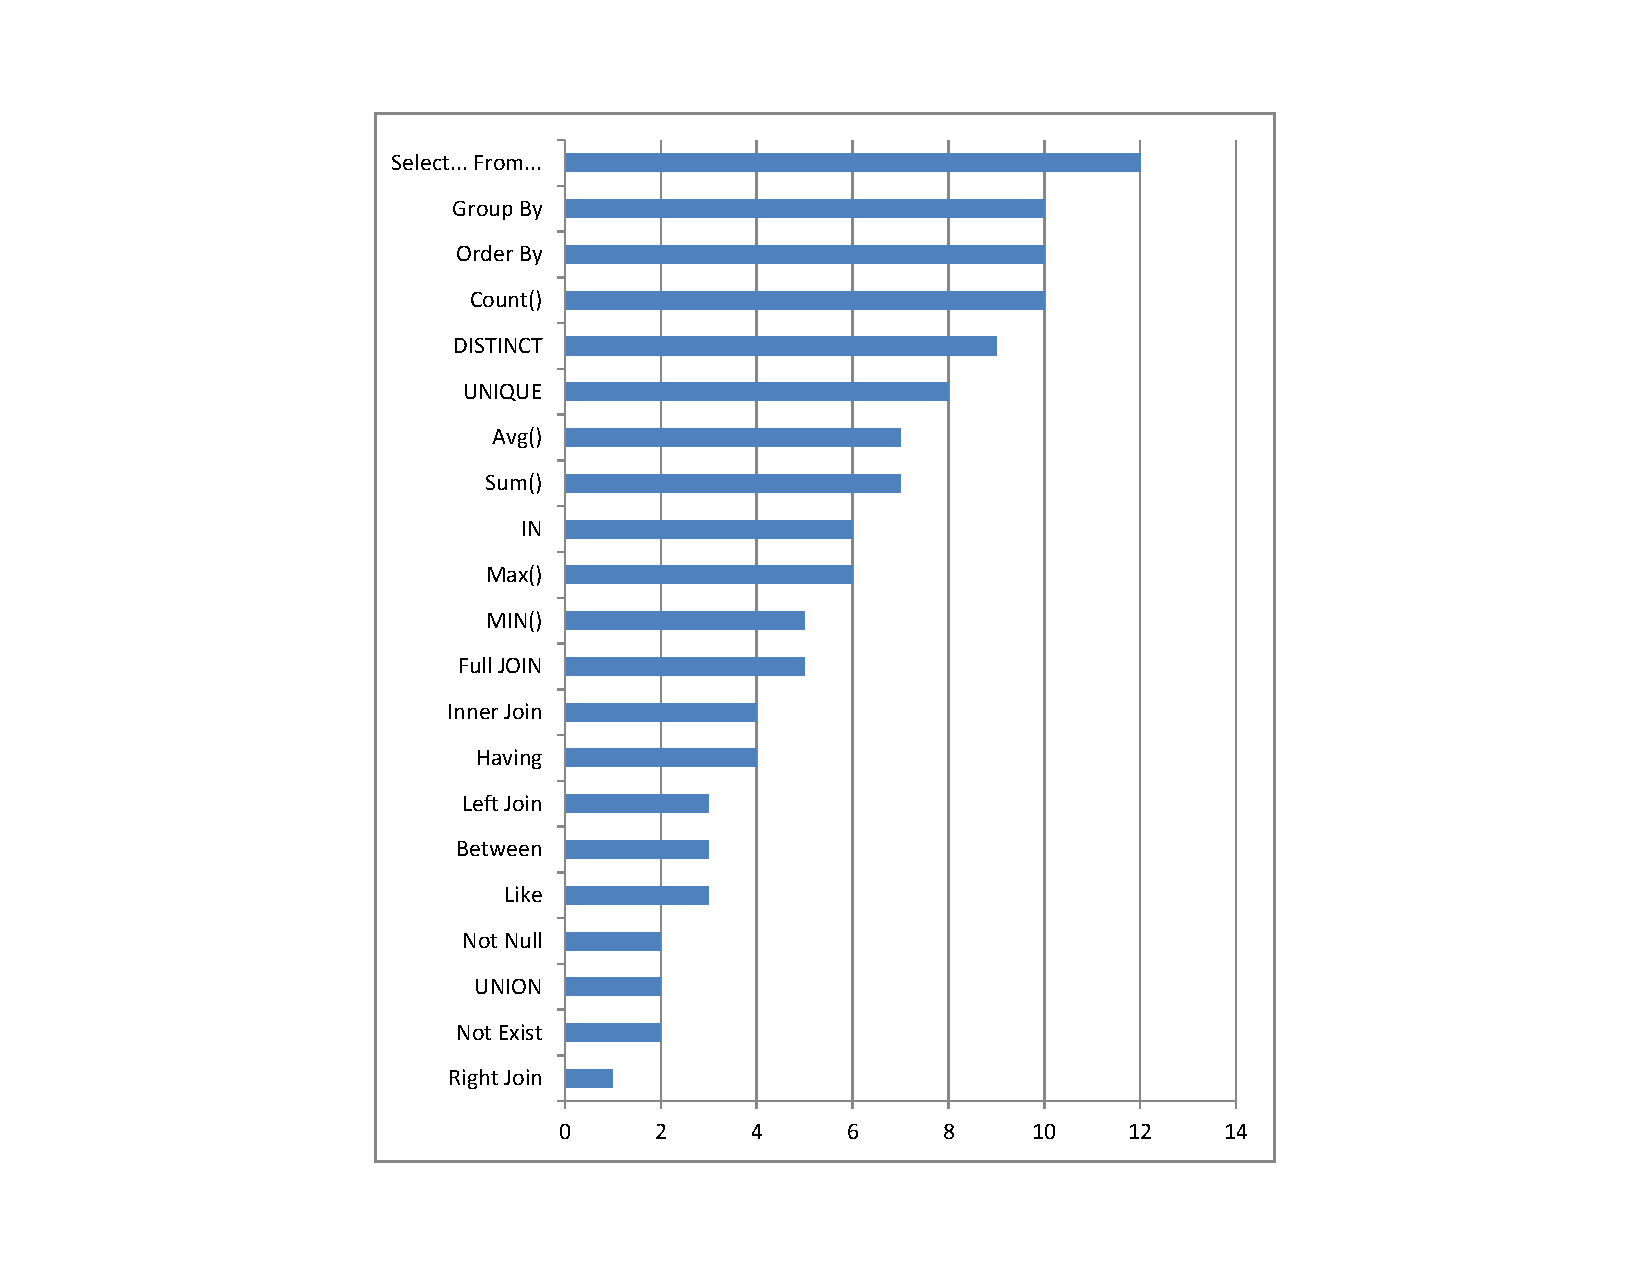
\includegraphics[scale=0.45]{survey}
  \vspace*{-3.0ex}\caption {{\label{fig:survey}
  Survey results of the most widely-used SQL features
  in writing a database query. 
 % There were 12 participants
 % in the survey, and each participant was asked to
 % select the top 10 widely-used SQL features.
  SQL features with no vote are omitted 
  for brevity.
}}
\end{figure}

\newcommand{\q}{\langle query\rangle}
\newcommand{\db}{\langle db\rangle}
\newcommand{\pat}{\langle pat\rangle}
\newcommand{\bug}{\langle bug\rangle}
\newcommand{\dist}{\langle distance\rangle}
\newcommand{\sem}[1]{\llbracket #1\rrbracket}
\newcommand{\lit}[1]{\texttt{#1}}

\newcommand{\column}{\langle column\rangle}
\newcommand{\dbtable}{\langle table\rangle}
\newcommand{\cond}{\langle cond\rangle}
\newcommand{\op}{\langle op\rangle}
\newcommand{\e}{\langle expr\rangle}
\newcommand{\ce}{\langle cexpr\rangle}

\begin{figure}[t]
%\scriptsize{%
\footnotesize%
\begin{align*}
\q ::= {} 
	& \texttt{ SELECT } \e^+ \texttt{ FROM } \dbtable^+ \\
        & \texttt{ WHERE } \cond^+ \\ 
	&  \texttt{ GROUP BY } \column^+ \texttt{ HAVING } \cond^+\\
	&  \texttt{ ORDER BY } \column^+ \\
\dbtable::= {} &\ atom \\
\column ::= {} &\ \dbtable.atom\\
\cond ::= {} &\ \ \cond \;\texttt{\&\&}\; \cond \\ 
    & |\ \cond \;\texttt{||}\; \cond \\
    & |\ \texttt{(}\;\cond\;\texttt{)} \\
    & |\ \ce \;\op\; \ce \\
\op ::= {} &\ \ \texttt{=} \;\;|\;\; \texttt{>}  \;\;|\;\; \texttt{<}\\
\ce ::= {} &\ \ const \;\;|\;\; \column  \;\; \\
\e ::= {} & \ce \;\;|\ \texttt{COUNT}(\column) \;\;|\ \texttt{COUNT}(\texttt{DISTINCT}\;\column)\\
    & |\ \texttt{SUM}(\column) \;\;|\ \texttt{MAX}(\column) \;\;|\ \texttt{MIN}(\column) 
\end{align*}
\normalsize%
\caption{Syntax of the supported SQL subset in \ourtool:
\textit{const} is a constant value and
\textit{atom} is a string value, representing
a table name or a column name.
%This subset covers the top XXX \todo{refer to figure 2}
%in Figure~\ref{fig:survey}
}
\label{fig:syntax}
\end{figure}


\section{A SQL Subset Supported in \ourtool}
\label{sec:langsubset}

%The problem of finding a SQL query satisfying
%an example input and output pair is PSPACE-hard~\cite{DasSarma:2010}. 
%To make it tractable,
%instead of supporting all features in the standard
%SQL language, 
\ourtool focuses on a widely-used SQL subset
using which a large class of query tasks can be performed.
Unfortunately, when designing the SQL
subset, we found that no empirical
study has ever been conducted to this end,
and little evidence has ever been provided
on which SQL features are widely-used in practice.
Without such knowledge, deciding which
SQL subset to support remains difficult.


To address this challenge and reduce our personal bias
in designing the language subset, we first conducted an online survey
to ask experienced IT professionals about the most widely-used
SQL features in writing database queries (Section~\ref{sec:survey}).
Then, based on the survey results, we designed
a SQL subset (Section~\ref{sec:syntax}).  
Later, we sent the designed SQL subset to the survey participants
and conducted a series of follow-up email interviews
to confirm whether our design would be sufficient in practice.




%Identify a domain of data on which a large class of users struggle to perform repetitive operations that they can clearly describe with examples





\subsection{Online Survey: Eliciting Design Requirements}
\label{sec:survey}


Our online survey consists of 6 questions that can be
divided into three parts. The first part includes
simple demographic questions about participants.
In the second part, participants are asked to select
the top 10 most widely-used SQL features in their minds.
Instead of directly asking participants about the SQL
features, which might be vague and difficult to respond,
we present them a list of \textit{all} standard
SQL features in writing a query.
Additionally, participants are asked to report their 
own experience in using SQL in the third part of the survey.

%Before distributing our survey, we conducted pilot
%interviews with three graduate students with XXX experience
%at University of Washington. We ran the survey with them and
%made notes of their comments. According to their feedback,
%we refined the survey questions and adjusted the wording to
%make sure that the questions are relevant and clear.


We sent out invitation to the graduate students at
University of Washington, and posted our survey on
professional online forums (e.g., StackOverflow).
As of April 2013, we received \respnum responses.
On average, the respondents had 9.5 years of experience
in software development (max: 15, min: 5),
and 5.5 years of experience in
using database (max: 10, min: 2). In addition, two
participants identified themselves as database professionals.
Figure~\ref{fig:survey} summaries the survey results.
% about
%the most-widely used SQL features rated by 12 participants.

\subsection{Language Syntax}
\label{sec:syntax}

Based on the survey results, we design a subset
of the standard SQL language, whose
syntax is shown in Figure~\ref{fig:syntax}.
%Its semantics are the same as the standard SQL language,
%and are omitted here for brevity.
%shown in
%that can contains
%many widely-used features required by real users. 
% shows the language syntax.


The supported SQL subset covers all top 10 most widely-used SQL
features voted by the survey participants
in Figure~\ref{fig:survey}, except for the \CodeIn{IN} keyword.
In addition, the SQL subset supports the \CodeIn{HAVING}
keyword since \CodeIn{HAVING} is often used together with the \CodeIn{GROUP BY} clause.
Our SQL subset, though by no means complete in writing all
possible queries, has significantly
enriched the SQL subsets supported by the existing query inference
work~\cite{DasSarma:2010, Tran:2009}. Besides being able to write the
standard select-from-where queries as in~\cite{DasSarma:2010, Tran:2009},
our SQL subset also supports table joins, aggregates
(e.g., \CodeIn{COUNT}, \CodeIn{MAX}, \CodeIn{MIN}, and \CodeIn{AVG}),
the \CodeIn{GROUP BY} clause, the \CodeIn{ORDER BY} clause,
and the \CodeIn{HAVING} clause. For readers who are not
familiar with the basic SQL idioms, we show an example query
using our SQL subset in Figure~\ref{fig:queryex}, and annotate
it with important concepts.


When designing the SQL subset, we focused on standard
SQL features, and excluded user-defined functions and
vendor-specific features, such as the \CodeIn{TOP}
keyword supported in Microsoft SQLServer. 
We discarded some standard SQL features, primarily for
three reasons. First, some features are designed
as syntactic sugar to make a SQL query easier to write;
and thus can be safely removed without affecting a language's
functionality. For example, the \CodeIn{BETWEEN}
keyword checks whether a given value is within a specific
range, and can be simply replaced by two query conditions.
Similarly, the \CodeIn{NOT NULL} keyword is also omitted.
%and \CodeIn{LIKE} keywords are also discarded.
Second, some features, such as 
\CodeIn{FULL JOIN}, \CodeIn{LEFT JOIN}, and \CodeIn{RIGHT JOIN},
provide special ways to join tables, and are less likely to be
used by non-expert end-users.
Third, other features, such as \CodeIn{IN}, \CodeIn{UNION}, and \CodeIn{NOT EXIST},
are used to write sub-queries or nested queries, which are the major source
of the PSPACE-hardness in query inference~\cite{DasSarma:2010}.
Related, the \CodeIn{LIKE} keyword is designed for string
wildcard matching; determining its matching
patterns requires systematic search and can be
expensive in practice. Thus, 
for the sake of inference efficiency, we exclude these keywords.

%would quickly become intractable during 
%pattern matching
%and can introduce unmanageable overhead during inference. 
%in order to make the synthesis problem more tractable.

%is also discarded, since it is used for
%string wildcard matching, and can also lead to \todo{xx}

%designed for 
%for the sake of The \CodeIn{LIKE}
%keyword is designed for string wildcard matching rather than
%table query. We also exclude it in the SQL subset




\subsection{Follow-up Interviews: Feedback about the SQL Subset}
\label{sec:interview}

After proposing the SQL subset in Figure~\ref{fig:syntax},
we performed follow-up email interviews to gain
participants' feedback about it. Participants were first asked to rate
the sufficiency of the SQL subset in Figure~\ref{fig:syntax}
in writing real-world database queries,
on a 6-point scale (5-completely
sufficient; 0-not sufficient at all;
and in-between values indicating intermediate sufficiency),
and then to provide their comments.

The average rating of the proposed SQL subset is 4.5. Most of
the participants rated it 5, or 4. Only one participant rated
it 3, because this participant misinterpreted the language
syntax and thought it does not support table joins.
%One participant commented that the SQL subset did not support
%column re-naming. However, re-naming database columns is not
%critical in sythesizing a correct SQL query \todo{xxx}

Overall, based on the feedback by experienced IT professionals,
we believe our SQL subset is usable
for end-users in writing common database queries.
%contains adequate SQL features
%in writing database queries that most end-users need.

\begin{figure}[t]
  \centering
  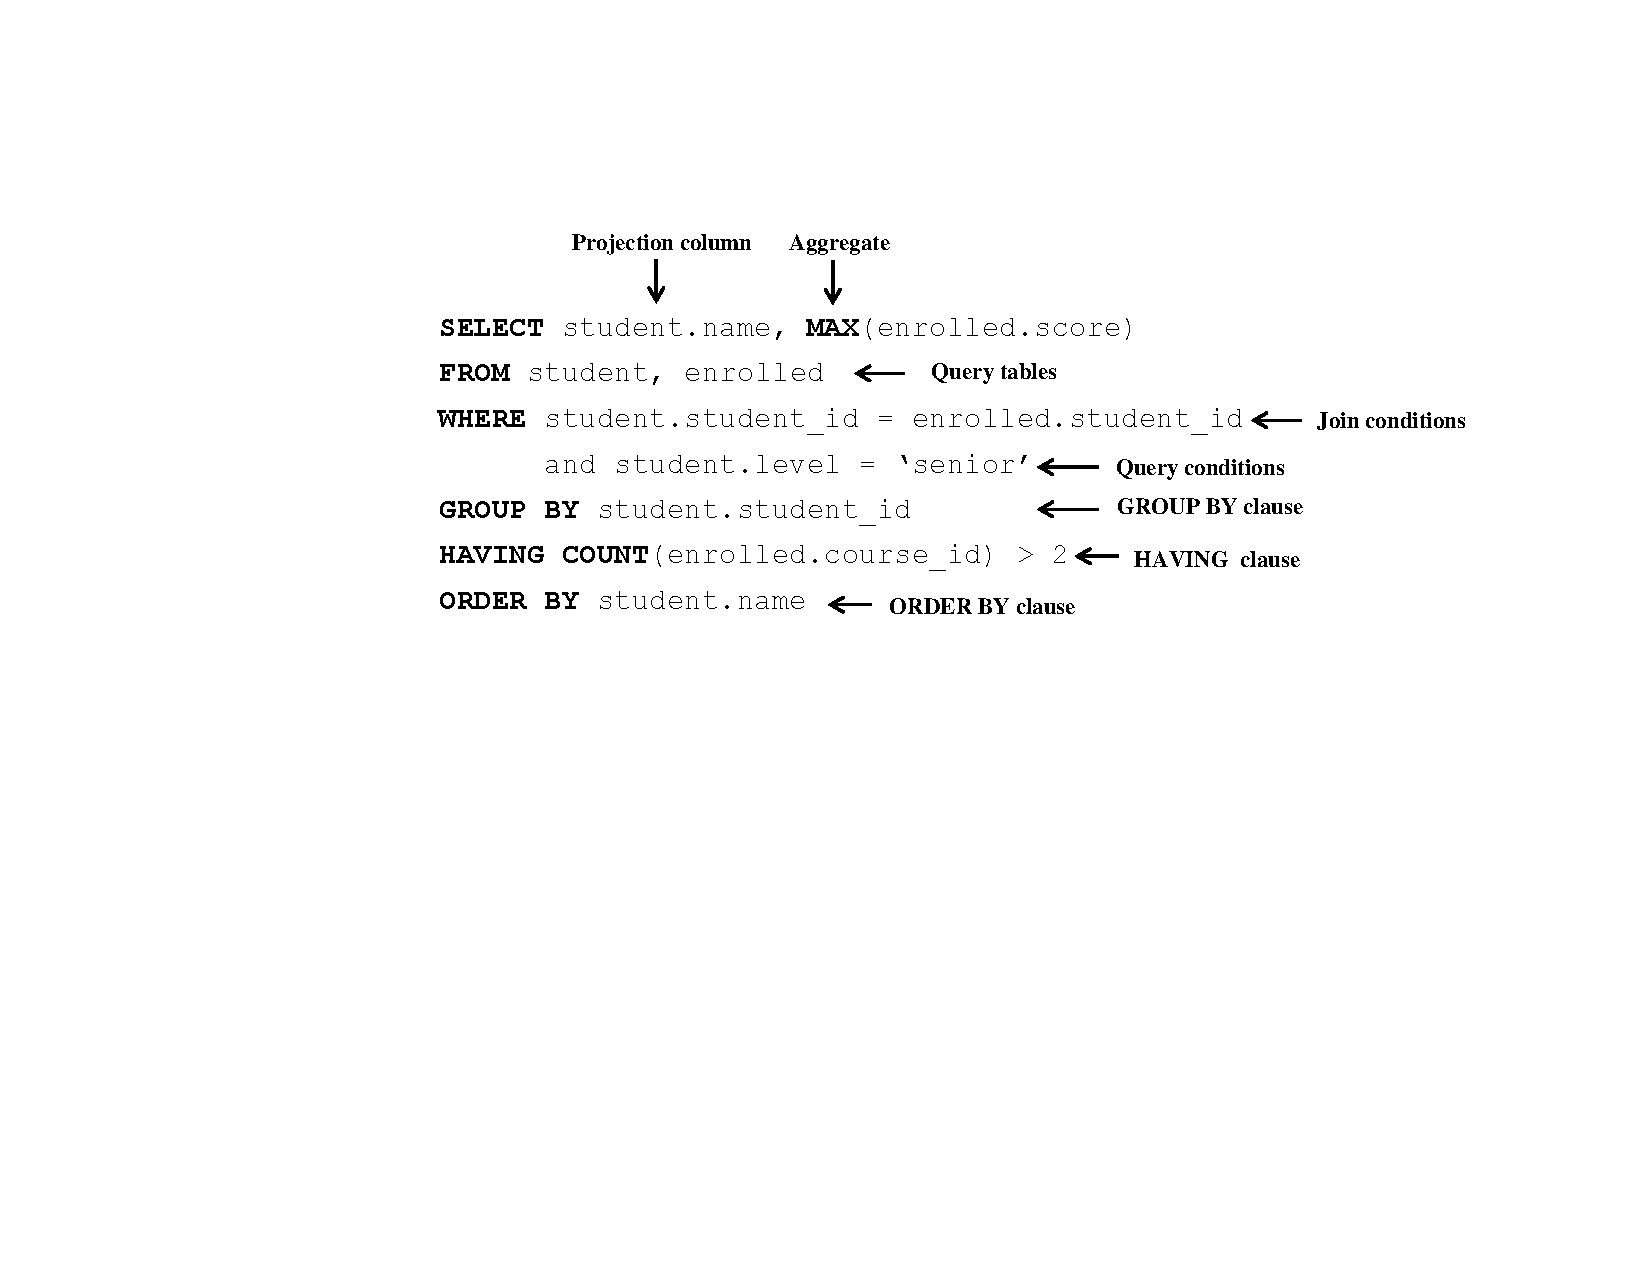
\includegraphics[scale=0.52]{queryex}
  \vspace*{-5.3ex}\caption {{\label{fig:queryex}
  An example query using the SQL subset defined in Figure~\ref{fig:syntax}.
}}
\end{figure}



\section{Technique}
\label{sec:approach}



We next describe our SQL query synthesis technique in detail.
How to infer the desirable query for the examples
shown in Section~\ref{sec:example} will
be discussed thoroughly in this section.

\begin{figure}[t]
  \centering
  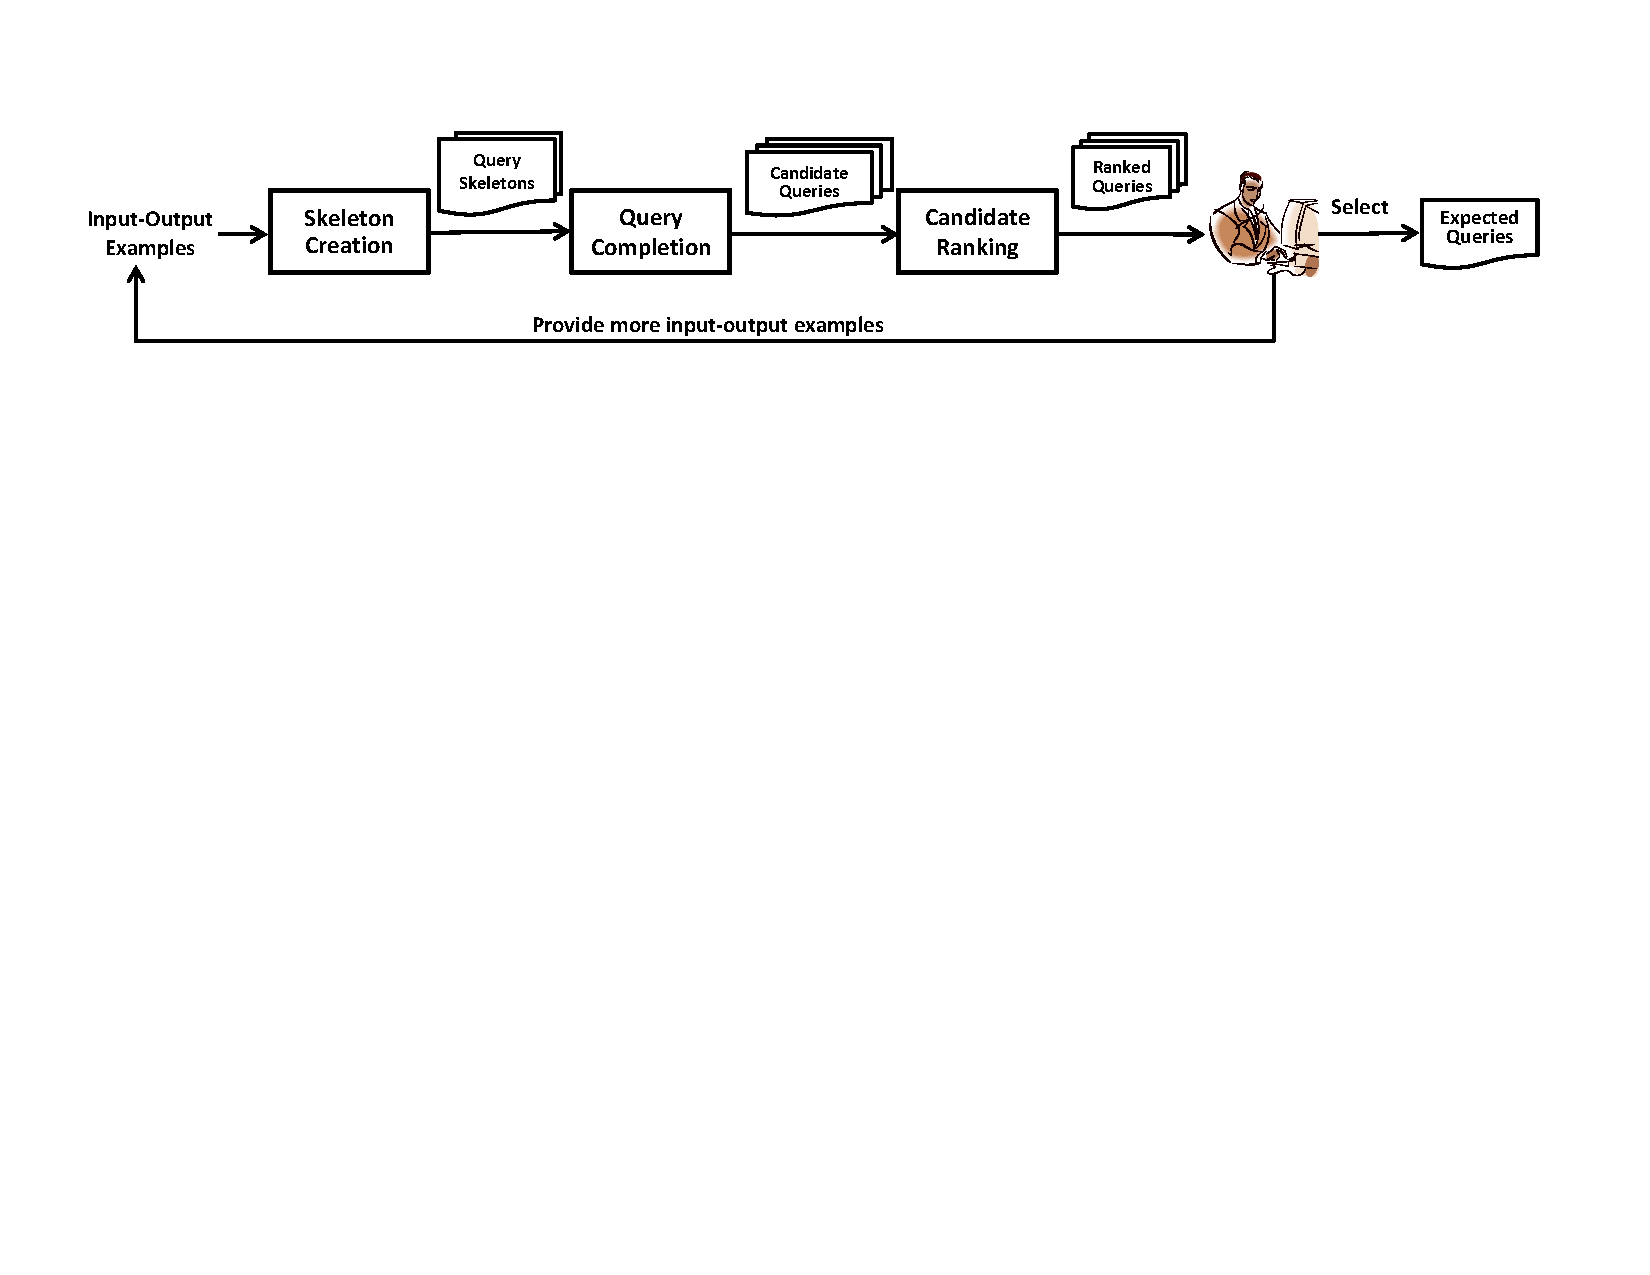
\includegraphics[scale=0.53]{workflow}
  \vspace*{-5.0ex}\caption {{\label{fig:workflow} The workflow of our SQL query synthesis approach.
}}

\end{figure}

\subsection{Overview}
Figure~\ref{fig:workflow} sketches the general workflow of our technique.

At a high level, our technique consists of three major steps: Query Skeleton
Creation(Section~\ref{sec:skeleton}), SQL Query Completion
(Section~\ref{sec:completion}), and Query Candidate Ranking (Section~\ref{sec:ranking}).
Specifically, our approach takes from users input-output examples. It first infers
a partially-complete query skeleton. The inferred query skeleton, though contains
incomplete parts that can not be yet decided, serves as a good reference
for further synthesizing a complete SQL query.
After that, our technique uses two techniques to complete a SQL skeleton.
In particular, it uses an advanced rule learning algorithm from the machine
learning community to infer query conditions (Section~\ref{sec:decision_tree}), and
 employs type-directed search to figure out possible aggregation
expressions (Section~\ref{sec:agg_search}).
The SQL Query Completion step produces a list of syntactically-valid
query candidates that satisfy the provided input-output examples.
However, it is possible that multiple query candidates can be synthesized based on the
provided input-output example. To deal with that, our technique
ranks all generated candidates,
and provides users a ranked list of SQL queries with the
simplest ones on the top. 
%This makes our tool more usable.


End-users can use our approach to obtain SQL query to transform
multiple, huge database tables by constructing small, representative
input and output example tables. On some examples, we speculate
that our approach
may produce a SQL query that satisfies the input and output examples
given by the user, but does not address the intention
that the user wants. To address this issue, we adapt a simple
interaction model from~\cite{Harris:2011} to ask users to investigate the results of
an output SQL query and report any discrepancy. In this case,
the user can refine the inferred SQL query by providing a more
informative input-output example (or multiple input-output examples
that together describe the required behavior) that demonstrate the behavior on
which the originally-inferred SQL query behaves incorrectly.

\subsection{Query Skeleton Creation}
\label{sec:skeleton}

In this step, our technique scans the provided input and output examples, guesses
what a target SQL query might look like, and infers a set of query skeletons
that capture the basic query structures.

A query skeleton is an incomplete SQL query, which
captures three basic query structures that could
often be decided after a simple scan over the examples:
tables used in a result SQL
query, table columns used to join input tables, and table
columns for projecting the query results. Other parts in a SQL query such as conditions
(including selection and having conditions), and aggregates
are left as unkown, and will be determinated in the next step (Section~\ref{sec:completion}).



%\begin{itemize}

%\item
\vspace{1mm}
\noindent \textit{\textbf{Step 1: Determining the Table Set.}} 
In practice, end-users are unwilling to provide more than enough
inputs. Therefore, every input table specified in the example
is expected to be used to construct a desirable SQL query.
Based on this observation, we assume that every input table
should be used as least once in the query. By default, the
table set $T$ used in the result SQL query contains all given input tables.
However, it is possible that a single table will be used for multiple times.
Our technique does not forbid this case, rather, we adopt a single heuristic
to estimate the used table set: if the same column from an input table appears more than once in the
example output, we add the input table the same number of times to the used table set.

%we view it as a strong indicator that this table will be joined multiple times and add it to our table
%set $T$ using an alias.


%\item
\vspace{1mm}
\noindent\textit{\textbf{Step 2: Determining Joining Columns. }} Given two arbitrary tables, there exist many
ways to join them. Enumerating all possible joining conditions may introduce a huge number of joining
conditions and would quickly become intractable. We observe that, in practice, two tables are often joined via the following
three cases: (1) tables are joined on their primary keys with the same (or compatible) data types, such
as joining a \textit{student} table with an \textit{enrollment} table with the \textit{student\_id} column. It does not
make any sense to join two tables on a Integer column and a String column. (2) tables are joined
using columns with the same name, such as joining a \textit{student} table with a \textit{enrollment} table on the
\textit{student\_name} column. and (3) two columns that have the data type, and have a large portion of
overlapped values in their corresponding input tables can be used as a joining condition. It is straightforward to check the first 
two cases to identify possible joining columns. For the third case, our technique scans the given input tables to check ``value similarity''
between two arbitrary columns, and selects columns whose ``value similarity'' is above a fixed threshold as joining columns.

%\item
\vspace{1mm}
\noindent \textit{\textbf{Step 3: Determining Output Columns.}} To identify output table columns on
which the querying result would be projected, our technique checks whether each output
table column name appears in any input tables. If so, we used the matched column
from the input table as the output column. Otherwise, the output column
must be produced by using aggregation. Our technique keeps track of those aggregation columns
and search for proper aggregates in the next phase (Section~\ref{sec:agg_search}). 

%After determining the table set and joining columns,
%the next step is to identify potential column names on which the result would be projected. If a
%column in the output table  does not appear in any input table's column list, this output column must
%be produced by aggregation. Our algorithm keeps track of these columns and appends a \CodeIn{group by} ... \CodeIn{having} ...
%clause to the query skeleton.

%\end{itemize}
\vspace{1mm}

In summary, this step infers three parts as a query skeleton: tables used in constructing a SQL query, joining conditions
to connect the input tables, and a list of columns to project the output results.

%It is worth noting that the results obtained from the above steps are not \textit{safe} in
%terms that they may miss some valid SQL queries. 

%We made the above assumption for the sake of tractability,
%since in theory, the bound of table number in a SQL query is $O(n_t!)$, where $n_t$ is the number of given tables;
%while the bound of possible number of join is $O(c_t^2)$ and the bound of the number of conditions is $O(n_t!n_tc_t^2)<O(n_t^3c_t^2)$.

%\subsubsection{Inferring Output Table Schema}

%Lacks schema

\subsubsection{Example}

For our motivating example, from the output table (Figure~\ref{tbl:output}), our technique identifies that
column {\CodeIn{Student\_name}} comes from table \CodeIn{student} and
column {\CodeIn{Max\_Score}} is a new one which must be created by using aggregation.
% which indicates aggregation and group by.

%while the bound of possible number of join is $O(c_t^2)$ and the bound of the number of conditions is $O(n_t!n_tc_t^2)<O(n_t^3c_t^2)$.

\begin{figure}[t]
	\centering
%\begin{CodeOut}
%\begin{alltt}
%\textbf{select student.Student\_name, $\color{blue}{<Aggregate>}$ 
%from student, enrolled
%where student.Student\_key = course.Student\_key
%      and \color{red}{<Conditions>}
%group by student.Student\_key
%having \color{red}{<Conditions>}}
%\end{alltt}
%\end{CodeOut}
%\vspace{-5mm}
		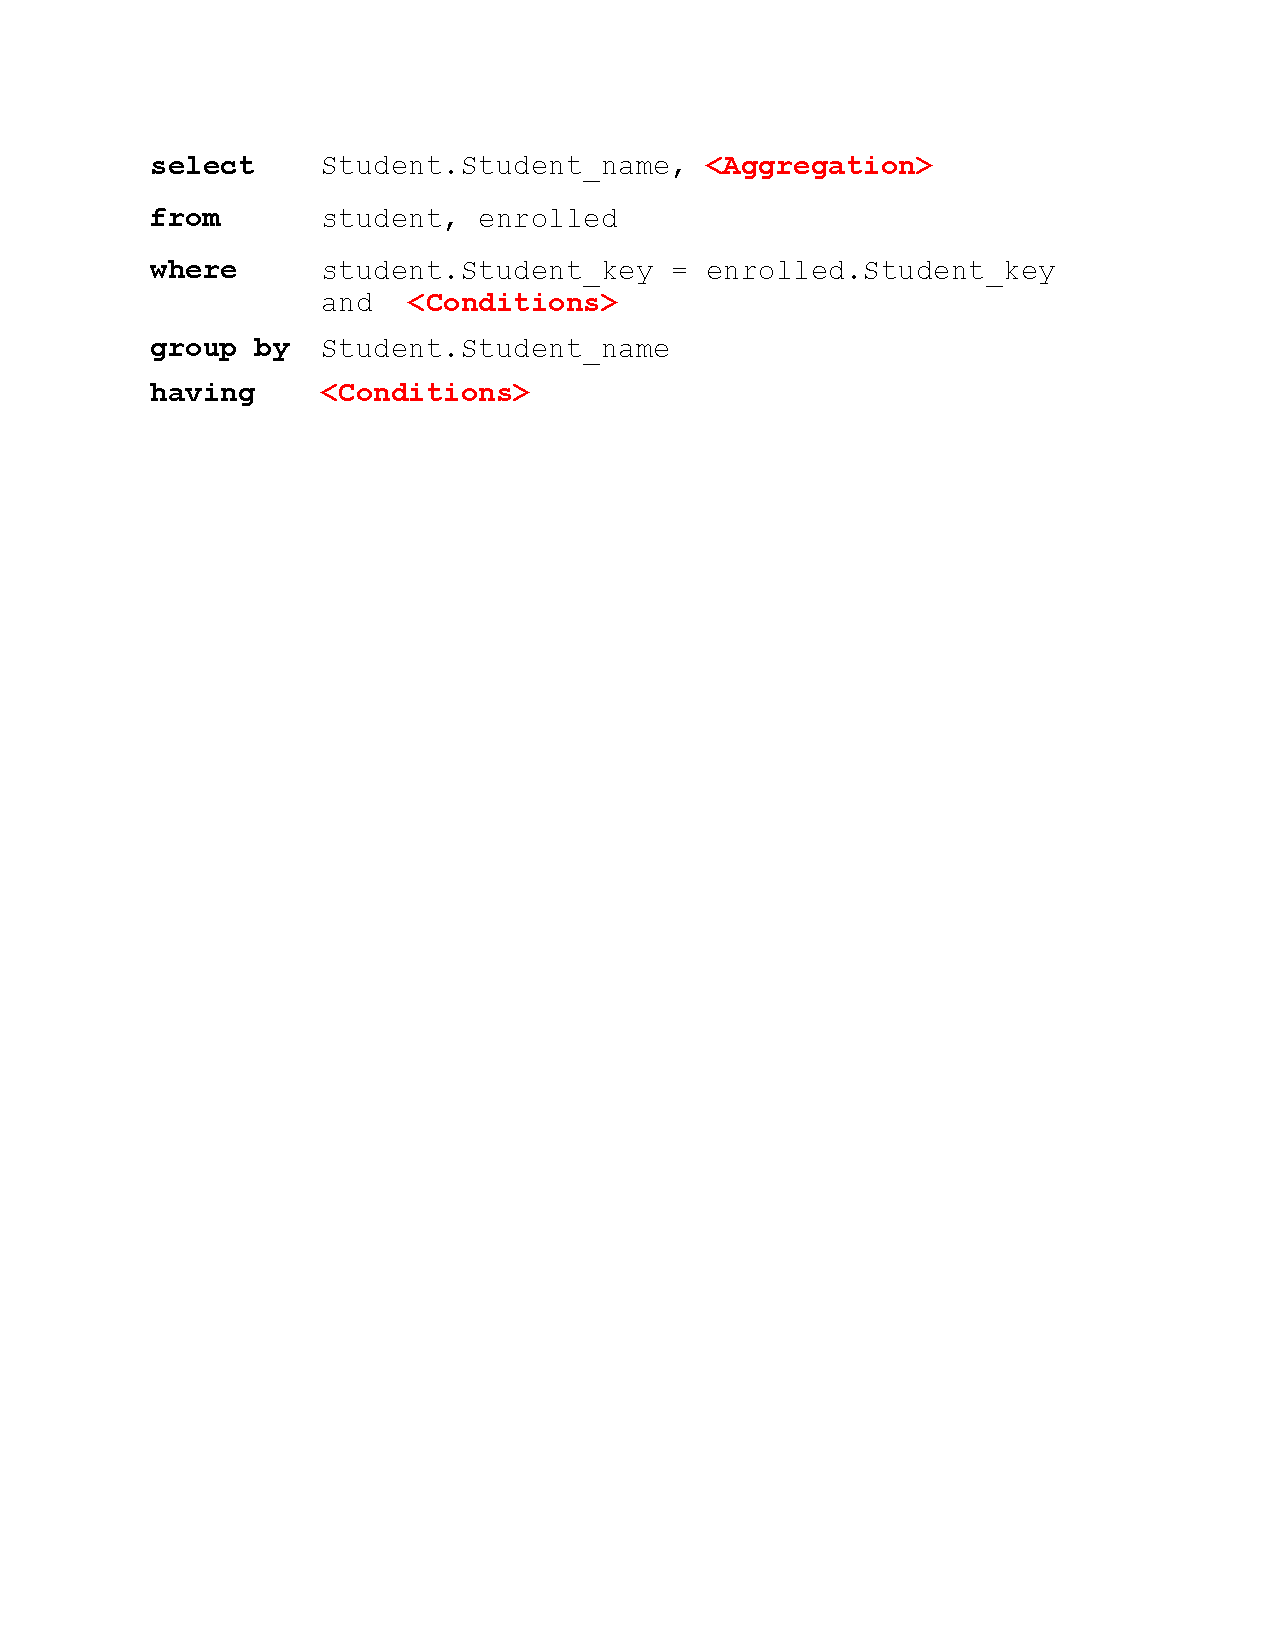
\includegraphics[width=0.4\textwidth]{sql_skeleton.pdf}
	\caption{The SQL skeleton created for the motivating example
in Section~\ref{sec:example}.}
	\label{fig:skeleton}
\end{figure}

The created query skeleton  is shown in Figure \ref{fig:skeleton}.
As we can see from Figure \ref{fig:skeleton},  there are three unknown structures represented
by $<$Aggregation$>$ or $<$Conditions$>$ in red color, which will be filled in the next phase.


\subsection{Query Completion}
\label{sec:completion}

\begin{figure*}[t]
    \centering
    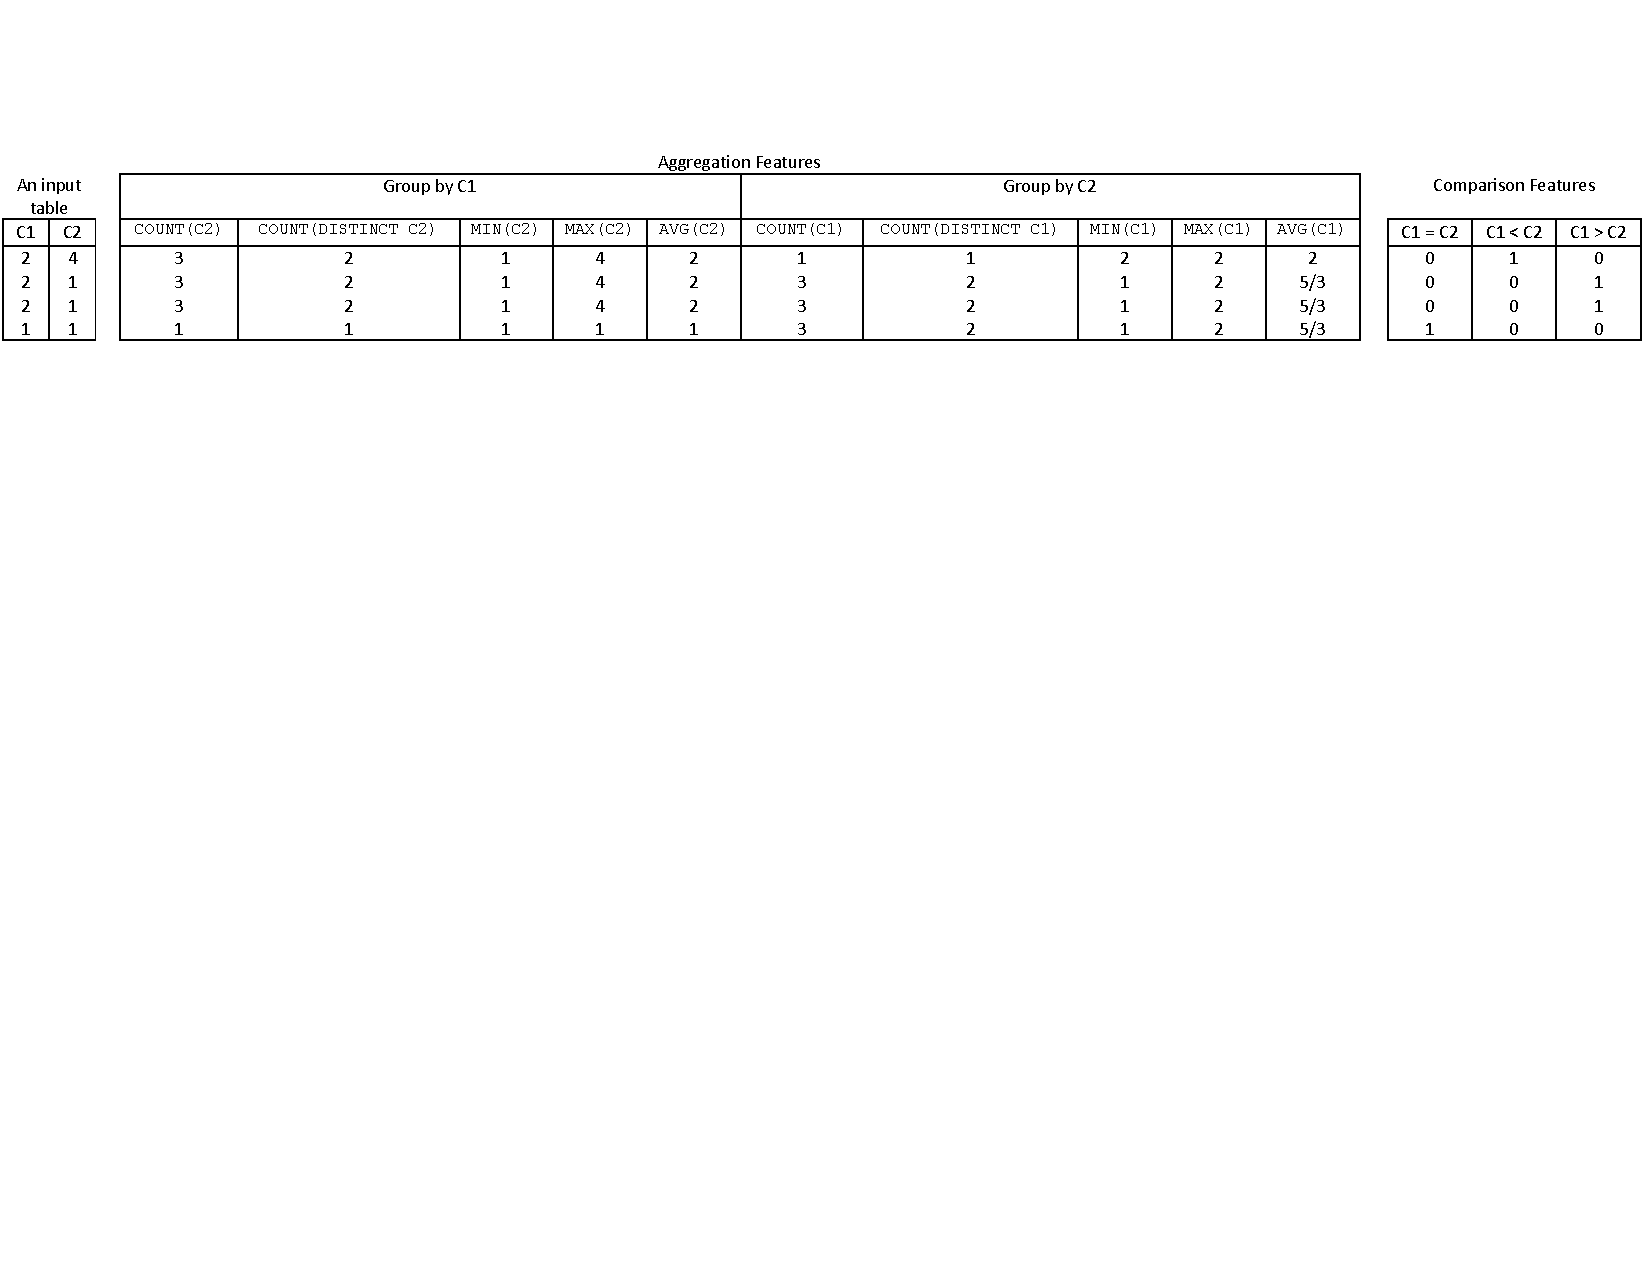
\includegraphics[scale=0.68]{featurex}
    \vspace{-7mm}
	\caption{Illustration of two additional features
    added by \ourtool. (Left) An example input table with
    two columns: C1 and C2. (Center) The aggregation features added by
    \ourtool for the input table. (Right) The comparison features
    added by \ourtool for the input table.
    Take the first row in the input table as an example,
    when grouping the table by column C1 (with value 2), the number
    of values in the C2 column is 3; the  number of
    distinct values in the C2 column is 2; the minimal value
    in the C2 column is 1, the maximal value in the C2 column
    is 4, and the average value in the C2 column is 2. Similar
    results can be computed if the table is grouped by the C2
    column.
}
	\label{fig:features}
\end{figure*}


In this step, \ourtool analyzes each created query skeleton
, and completes the missing query conditions, the
\CodeIn{GROUP BY} and \CodeIn{HAVING} clause (Section~\ref{sec:condition}),
aggregates (Section~\ref{sec:agg_search}), and
the \CodeIn{ORDER BY} clause (Section~\ref{sec:orderby}).
\ourtool outputs a list of syntactically-correct SQL queries
that satisfy the given example input and output.


%The SQL skeleton produced by the first step, though incomplete,
%serves as a good reference in inferring complete and valid SQL queries.
%In this step, our technique the remaining incomplete parts: conditions and
%aggregates, by rule-based learning and type-directed search, respectively.

\subsubsection{Inferring Query Conditions}
\label{sec:condition}

\ourtool casts the problem of \textit{inferring query conditions} as
 \textit{learning appropriate rules} that can perfectly divide a search space
into a positive part and a negative part. In our context, the search space
is all tuples from joining all query tables; the positive part
includes all tuples in the output table; and the negative part includes the rest
tuples.

The standard way for rule learning is using a decision-tree-based
algorithm. However, how to design a good features
becomes a key challenge.
Existing approaches~\cite{Tran:2009} simply use
tuple values in the input table(s) as features, 
and limits their abilities in inferring more
complex rules as query conditions. In particular,
merely using tuple values as features can only infer
conditions that compares a column value with a constant
(e.g., \CodeIn{student.level = 'senior'}), but
fails to infer conditions using aggregates (e.g., \CodeIn{COUNT(enrolled.course\_id) > 2}),
or conditions comparing the values of two table columns
(e.g., \CodeIn{enrolled.course\_id > enrolled.score}).



\ourtool addresses this challenge by adding two types of
additional features to each tuple, and uses
the existing tuple values together with the additional features
for rule learning.

\begin{itemize}

\item {\textbf{Aggregation Features}}. For each
column in an input table, \ourtool tries
to group all table data by \textit{each} tuple's
value, then applies every applicable aggregate (i.e.,
\CodeIn{COUNT}, \CodeIn{COUNT DISTINCT}, \CodeIn{MAX},
\CodeIn{MIN}, and \CodeIn{AVG} for a numeric type column;
and \CodeIn{COUNT}, and \CodeIn{COUNT DISTINCT} for
a string type column) to every
 \textit{remaining} column for computing the aggregation result. 
The ``Aggregation Features'' part in Figure~\ref{fig:features}
shows an example.

\item {\textbf{Comparison Features}}. For each tuple,
\ourtool compares
the values of every two type-comparable columns, and records
the comparison results ($1$ or $0$) as features.
The ``Comparison Features'' part in Figure~\ref{fig:features}
shows an example.

\end{itemize}

%The above two additional features seamlessly encodes SQL
%structure
% knowledge encoding permits our technique
%to make use of correlations between columns, rather than only values
%from each isolated and sequential columns.
%Table~\ref{tbl:com} shows an example.


%Using both tuple values and the enhanced features,
\ourtool employs a variant of the decision tree algorithm,
called PART~\cite{Frank:1998}, to learn a set of rules
as query conditions.
PART has two notable advantages over the
original decision tree algorithm~\cite{Quinlan:1986}.
First, it uses a ``divide-and-conquer'' strategy to repeatedly
build rules and remove data instances (i.e., tuples) that have already been covered until
no more data instances are left, and thus is faster.
Second, PART less memory, since it builds a decision
tree incrementally, prunes falsified branches on-the-fly,
and only keeps the minimal tree structure in memory.



\todo{The incerasing number of features, can be falsified quickly,
more features permits undiscover more rules}


Figure~\ref{fig:fullexample} shows an example, in
which the expected query condition uses the \CodeIn{COUNT} aggregate.


\begin{figure*}[t]
  \centering
  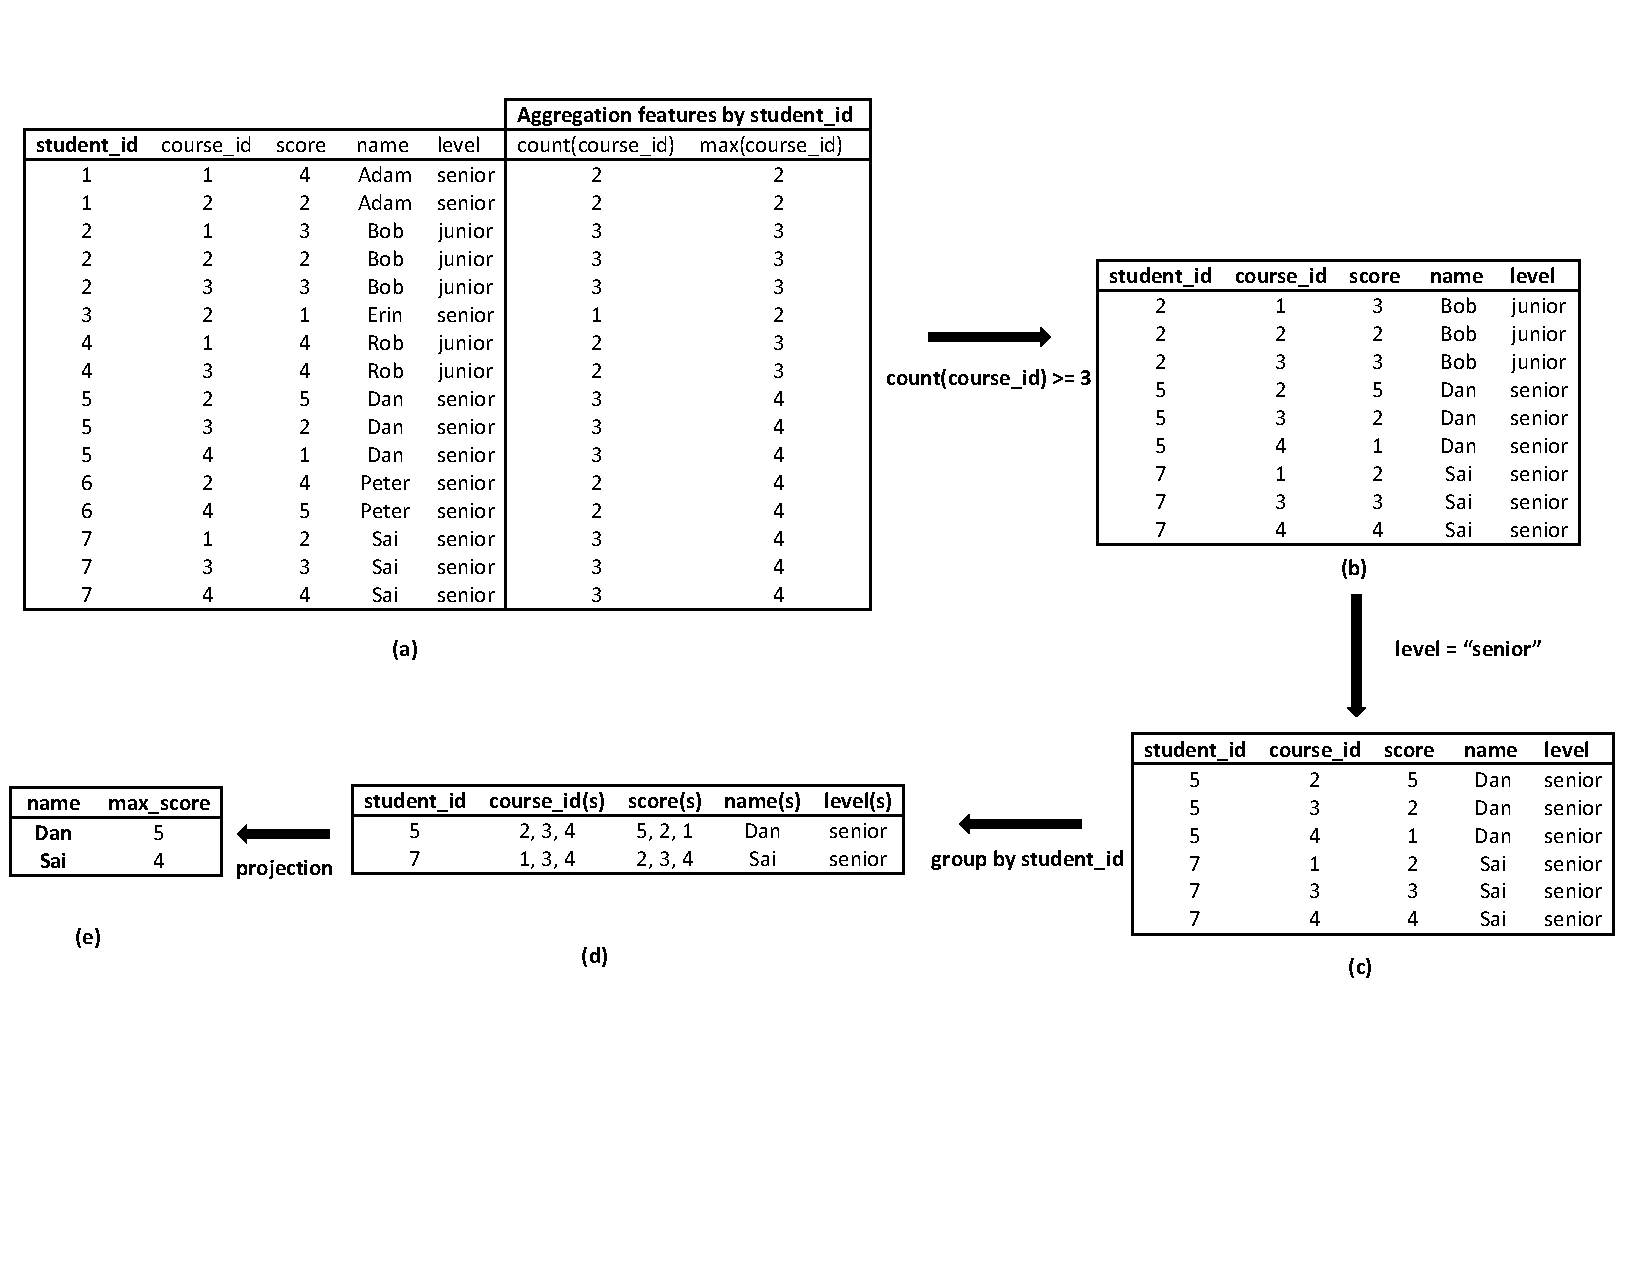
\includegraphics[scale=0.65]{fullexample}
  \vspace*{-5.0ex}\caption {{\label{fig:fullexample}
  Illustration of how additional features added by \ourtool
  helps in inferring query conditions. (a) shows \ourtool
  enriches the original table (Left: the
  result of joining table \CodeIn{student} with table
  \CodeIn{enrolled} on the \CodeIn{student\_id} column)
  with additional features. For brevity, only relevant
  aggregation features are shown. Using the added aggregation
  features, \ourtool infers two query conditions that
  transform the original table into the table show in (b).
  Note that, without the aggregation features enhanced by
  \ourtool, a learning algorithm will \textit{fail} to learn the above conditions.
  (c) shows the output table, which is produced by projecting the
   table in (b)
  on its column: name, and an aggregate: \CodeIn{MAX}(score).
}}

\end{figure*}


\ourtool next splits the learnt rules into two disjoint parts:
and put each part into its appropriate place.
Specifically, \ourtool puts conditions
using aggregates to the \CodeIn{HAVING}
clause; and puts other conditions to the \CodeIn{WHERE} clause.
This is based on the SQL language's specification:
query conditions using aggregates are valid only when they
are used \textit{after} the \CodeIn{GROUP BY} clause.
Take the conditions inferred in Figure~\ref{fig:fullexample}
as an example, \ourtool puts the query
condition: \CodeIn{student.level =`senior'}
in the \CodeIn{WHERE} clause,
puts condition: \CodeIn{COUNT(enrolled.course\_id) > 2}
in the \CodeIn{HAVING} clause, and puts
column \CodeIn{student\_id} to the \CodeIn{GROUP BY} clause.

%\smallskip





%\end{itemize}

\subsubsection{Searching for Aggregates}
\label{sec:agg_search}

For every column in the output table that has no matched
column in the input tables,
\ourtool repeatedly applies each aggregate on
every input table column; and then outputs the aggregate (with the
input table column) that produces the same output 
in the output table. To speed up the exhaustive search,
\ourtool uses two rules to filter away many infeasible
combinations.


\begin{itemize}
\item \ourtool only applies an \textit{applicable} aggregate
to a \textit{type-compatible} table column. Specifically,
the data values in an output column must be compatible with an
aggregator's return type. For instance, if an output column
contains float values, it cannot be produced by using the \CodeIn{COUNT}
or \CodeIn{COUNT DISTINCT} aggregators, or 
using the \CodeIn{MAX} aggregator over a column with integer type.
On the other hand, some aggregates cannot be applied on
table columns with certain types. For example, the \CodeIn{AVG}
aggregate cannot be applied to columns with string type.
%\ourtool encodes such knowledge to avoid unnecessary search.

\item \ourtool checks whether each value in the output
column has appeared in the input table. If not, the
output column cannot be produced by using
using the \CodeIn{MAX} and \CodeIn{MIN} aggregator.
%such as \CodeIn{MAX} and \CodeIn{min},
%is used, each value in the output column must has appeared in the input table.
\end{itemize}

%In our experience, the type-directed searching strategy significantly reduces the
%searching space and makes our tool find the desirable aggregates faster.

%\todo{Order by structure, relatively each to add}
\subsubsection{Searching for columns in the \CodeIn{ORDER BY} column}
\label{sec:orderby}
\ourtool scans the values of each column in the output table. If
the data values in a column are sorted, \ourtool
append the column name to the \CodeIn{ORDER BY} clause.


\subsection{Candidate Ranking}
\label{sec:ranking}


It is possible that multiple SQL queries satisfying
the given input-output examples will be returned.
To help end-users select their expected queries,
\ourtool ranks more likely queries higher in the output.
%This may adversely impact end-users who want to
%perform simple query tasks but now need
%to select the query of their intent.
%To alleviate this problem, 
To do so, \ourtool employs
the Occam's razor principle, which states that the
simplest explanation is usually the correct one.
A simpler query is less likely to overfit the given examples
than a complex one, even when both of them
can transform the example input to the example output.


%We define a comparison scheme between different
%SQL queries by defining a partial order between them. Some of
%these choices are subjective, but have been observed to work well.
A SQL query is simpler than another one if it uses
fewer query conditions (including conditions in the \CodeIn{HAVING}
and \CodeIn{FROM} clauses) or the expressions (including
aggregates) in each query condition or clause are pairwise simpler.
For example, expression \CodeIn{COUNT(student\_id)} is simpler than
\CodeIn{COUNT(DISTINCT student\_id)}.
Simpler query conditions and expressions often suggest the extraction logics
are more common and general.

In our implementation, \ourtool computes a cost for each
query, and prefers queries with lower costs. The cost
for a SQL query is computed by summarizing
the costs of all conditions, aggregates,
and other expressions
appearing in the \CodeIn{GROUP BY} and \CodeIn{ORDER BY} clauses.
(The cost of each condition, aggregate and expression
is approximated by its length.)
%This heuristic has been observed
%to work well.
Figure~\ref{fig:rank} shows an example.


\begin{figure}[t]
\centering
 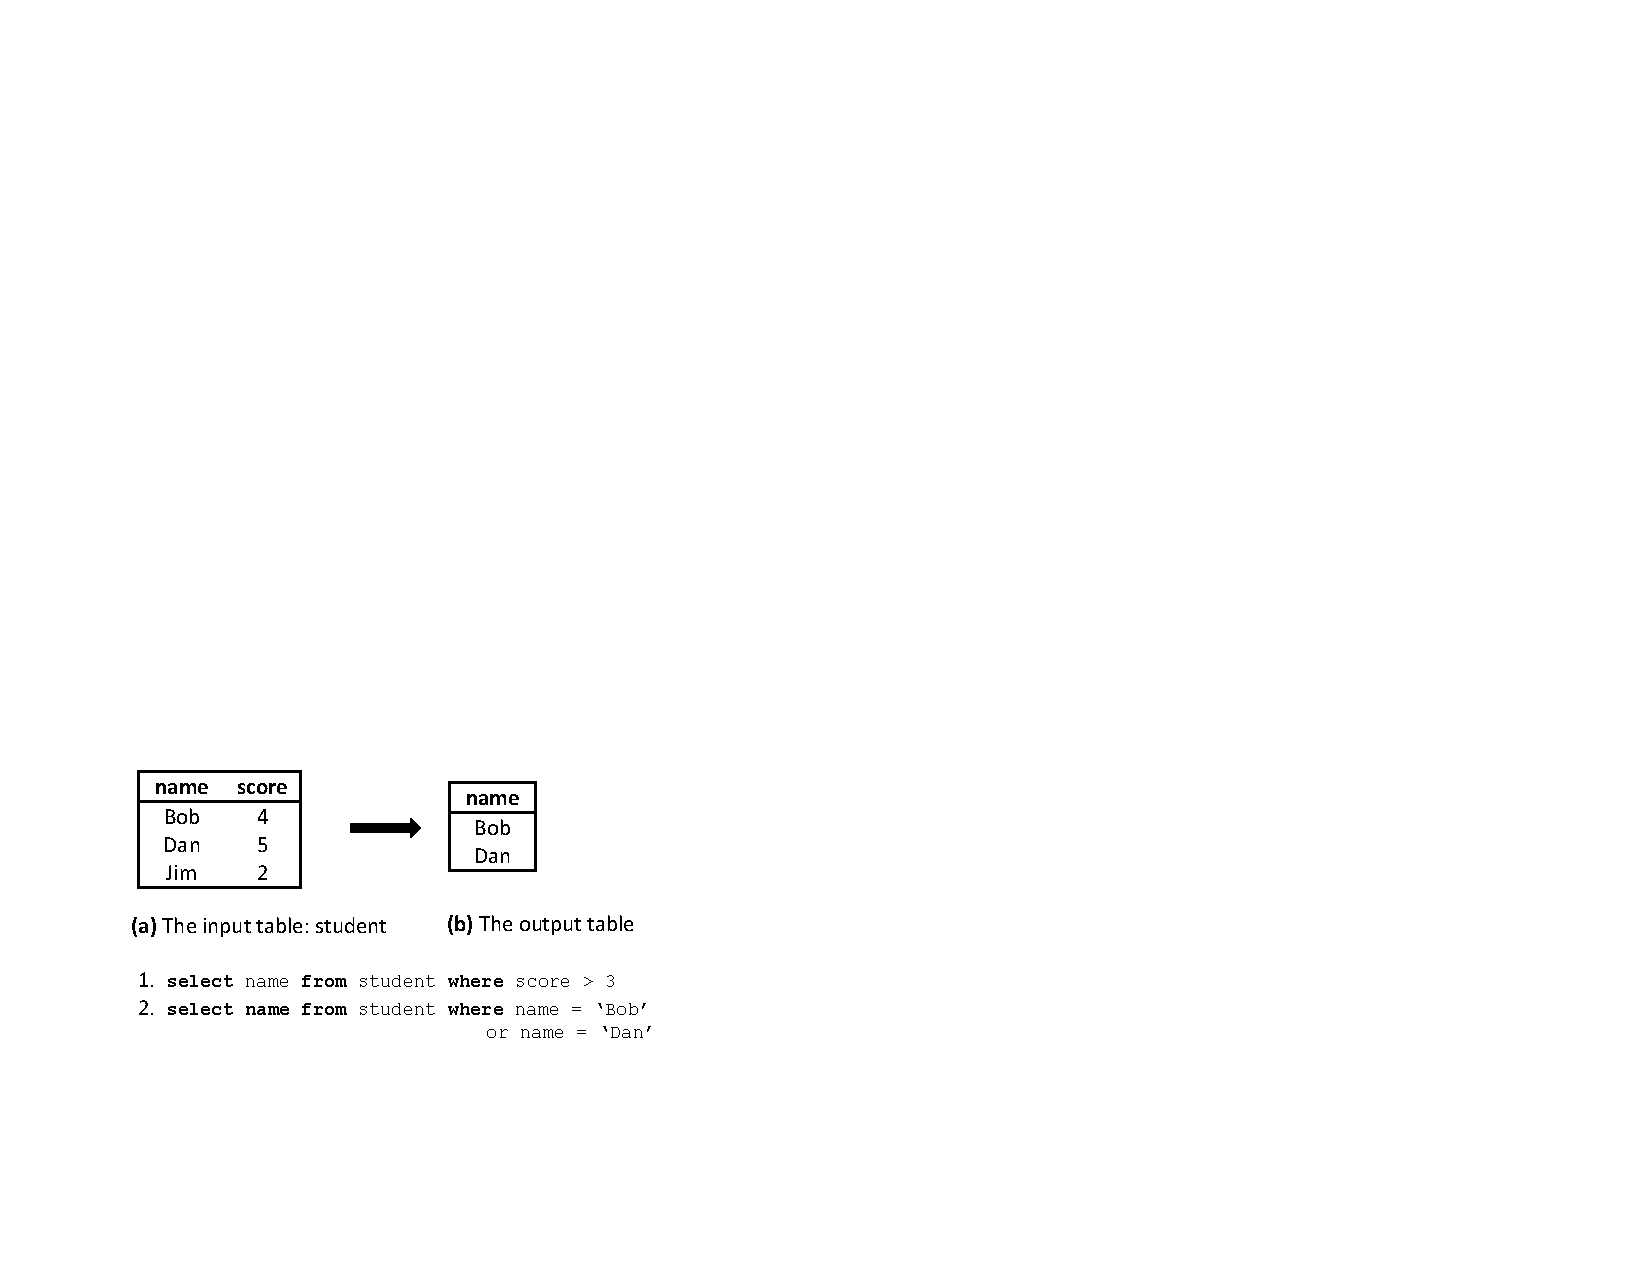
\includegraphics[scale=0.80]{rankexample}
 \vspace{-4mm}
\Caption{{\label{fig:rank} Illustration of \ourtool's
query ranking heuristic. \ourtool produces two
queries for the given examples. The first query
differs from the second query in using a simpler condition,
and thus is ranked higher.
}}
\end{figure}




%\subsection{User Interactive Model}
%\label{sec:uim}




%
\section{Implementation}
\label{sec:implementation}

We implemented the proposed technique in a tool, called \ourtool. 
\ourtool uses the built-in PART algorithm implementation in
the Weka toolkit~\cite{Hall:2009} to learn query conditions
(Section~\ref{sec:completion}). \ourtool also uses
MySQL~\cite{mysql} as the backend
database to validate the correctness of each synthesized 
SQL query. Specifically, \ourtool first populates the backend database
with the given input tables; when a SQL query is
synthesized, \ourtool executes the query on the database
to observe whether the output matches the given output.
Our implementation is publicly available at:
\url{http://sqlsythesizer.googlecode.com}

\pagebreak


\section{Evaluation}
\label{sec:evaluation}

We evaluated four aspects of \ourtool's effectiveness,
answering the following research questions:

\begin{itemize}
\item What is the success ratio of \ourtool in synthesizing
SQL queries? (Section~\ref{sec:ratio}).
%Is the supported SQL subset expressive enough to describe a variety of queries?
\item How long does it take for \ourtool to
synthesize a SQL query (Section~\ref{sec:performance}).
\item How much human effort is needed to write sufficient
input-output examples for SQL synthesis (Section~\ref{sec:human}).
\item How does \ourtool's effectiveness compare to
existing SQL query inference techniques (Section~\ref{sec:comparison}).
\end{itemize}






\subsection{Benchmarks}

We collected benchmarks from two sources:

\begin{itemize}
\item We selected \textit{all} SQL query related exercises
(\allex in total) from a classic database textbook~\cite{cowbook}.
All exercises are from Chapter 5, which systematically
introduces the SQL language.
Textbook exercises are good resource to evaluate \ourtool's
generality, since such exercises are often designed to
cover a wide range of SQL features. Some exercises
are even designed on purpose to cover some less realistic,
corner cases in using SQL. As shown in Figure~\ref{tab:results},
each textbook exercises involves at least 3 tables. It was unintuitive
for us to write the correct query by simply looking at the problem
description.

\item We searched SQL query related questions raised by real-world
database users from 3 popular online forums~\cite{stackoverflow, tutorialized, dbjournal}.
We focused on questions about using standard SQL features
rather than vendor-specific SQL features. We
excluded questions that were vaguely described or obviously
wrong, and discarded questions that had been proved
to be unsolvable by using SQL (e.g., computing a
transitive closure).
We collected \pnum recent forum questions related to writing a SQL query.
\todo{merge same types. exclude jdbc, why relative few}
\end{itemize}



\subsection{Evaluation Procedure}

We used \ourtool to solve each textbook exercise and forum
question. If an exercise or problem
was associated with example input and output,
we directly applied \ourtool on those examples.
Otherwise, we manually wrote some example input and output.
To reduce the bias in writing
examples, all examples are written by a graduate
student (whose research field is not database-related) from University of Washington rather than
\ourtool's developers.

We checked \ourtool's correctness by comparing its
output with the expected SQL queries.
For textbook exercises, we compared \ourtool's output with
their correct answers; for forum questions, we
manually wrote the correct SQL query and then
compared it with \ourtool's output.
%determined
%whether \ourtool can produce it.
%the output query can fulfill
%the query task or not.

For some textbook exercises and forum questions,
\ourtool inferred a SQL query that satisfied the input-output
examples, but did not behave as we expected when applied
to other inputs. We manually found another input on which the
SQL query mis-behaved and re-applied \ourtool to the new input. We
repeated this process and recorded the number of
interactions until \ourtool synthesized a correct SQL query.


All experiments were run on a 2.67GHz Intel Core PC
with 4GB physical memory (2GB was allocated for the JVM),
running Windows 7.



\begin{figure*}[t]
\setlength{\tabcolsep}{.24\tabcolsep}
\begin{tabular}{|c|l|c||c|c|c|c|c||l|}
\hline
\multicolumn{3}{|c||}{Benchmarks} & \multicolumn{5}{|c||}{\ourtool} & Query by\\
\cline{1-8}
 ID & Source & \#Input Tables & Example Size & Rank & Time Cost (s) & Cost in Writing Examples (m) & \#Iterations & Output~\cite{Tran:2009}\\
 \hline
 \hline
 1 &Textbook Ex 5.1.1 & 4 &  & & & & & \\
 2 &Textbook Ex 5.1.2 & 4&  & & & & & \\
 3 &Textbook Ex 5.1.3 & 4&  & & & & & \\
 4 &Textbook Ex 5.1.4 & 4&  & & & & & \\
 5 &Textbook Ex 5.1.5 & 4&  & & & & & \\
 6 &Textbook Ex 5.1.6 & 4&  & & & & & \\
 7 &Textbook Ex 5.1.7 & 4&  & & & & & \\
 8 &Textbook Ex 5.1.8 & 4&  & & & & & \\
 9 &Textbook Ex 5.1.9 & 4&  & & & & & \\
 10 &Textbook Ex 5.1.10 & 4&  & & & & & \\
 11 &Textbook Ex 5.1.11 & 4&  & & & & & \\
 12 &Textbook Ex 5.1.12 & 4&  & & & & & \\
 13 &Textbook Ex 5.2.1 & 3 &  & & & & & \\
 14 &Textbook Ex 5.2.2 & 3&  & & & & & \\
 15 &Textbook Ex 5.2.3 & 3&  & & & & & \\
 16 &Textbook Ex 5.2.4 & 3&  & & & & & \\
 17 &Textbook Ex 5.2.5 & 3&  & & & & & \\
 18 &Textbook Ex 5.2.6 & 3&  & & & & & \\
 19 &Textbook Ex 5.2.7 & 3&  & & & & & \\
 20 &Textbook Ex 5.2.8 & 3&  & & & & & \\
 21 &Textbook Ex 5.2.9 & 3&  & & & & & \\
 22 &Textbook Ex 5.2.10 & 3&  & & & & & \\
 23 &Textbook Ex 5.2.11 & 3&  & & & & & \\
 24 &Forum Question 1 & &  & & & & & \\
 25 &Forum Question 2 & &  & & & & & \\
 26 &Forum Question 3 & &  & & & & & \\
 27 &Forum Question 4 & &  & & & & & \\
 28 &Forum Question 5 & &  & & & & & \\
\hline
\end{tabular}
\Caption{{\label{tab:results} Experimental results of SQL query synthesis.
Column ``Benchmarks'' describes the characteristics of our benchmarks. Sub-column ``\#Input Tables''
shows the number of input tables in each benchmark. Column ``\ourtool'' shows
\ourtool's results. Sub-column ``Example Size''
shows the number of tuples (i.e., rows) in all example input and output tables.
Sub-column ``Rank'' shows the absolute
rank of the correct SQL query in \ourtool's output.
``\textbf{X}'' means \ourtool fails to produce a correct answer.
Sub-column ``Cost in Writing
Examples (m)'' shows the total time cost of writing sufficient
examples in minutes. Sub-column ``\#Iterations'' shows the number of
interactive rounds in using \ourtool to obtain the correct query.
Column ``Query by Output'' shows the results of using an existing
technique, called
\textit{Query by Output} (QBO)~\cite{Tran:2009}. In this column,
``\textbf{Y}''  means QBO produces the correct SQL query, and ``\textbf{N}''
means QBO fails to produce the correct query.
Since QBO was implemented as a special case in \ourtool; its
time cost is similar to \ourtool and is omitted for brevity.
}}
\end{figure*}



\subsection{Results}

Figure~\ref{tab:results} summarizes our experimental results.

\subsubsection{Success Ratio}
\label{sec:ratio}


As shown in Figure~\ref{tab:results}, \ourtool
synthesized expected SQL queries for \solexnum  out of
\exnum the textbook exercises, and \solpnum out of
\pnum the forum questions.
%per exercise (or problem).

\todo{why the technique can work, why some problem
can not be solved}

%

\begin{figure*}[t]
  \centering
  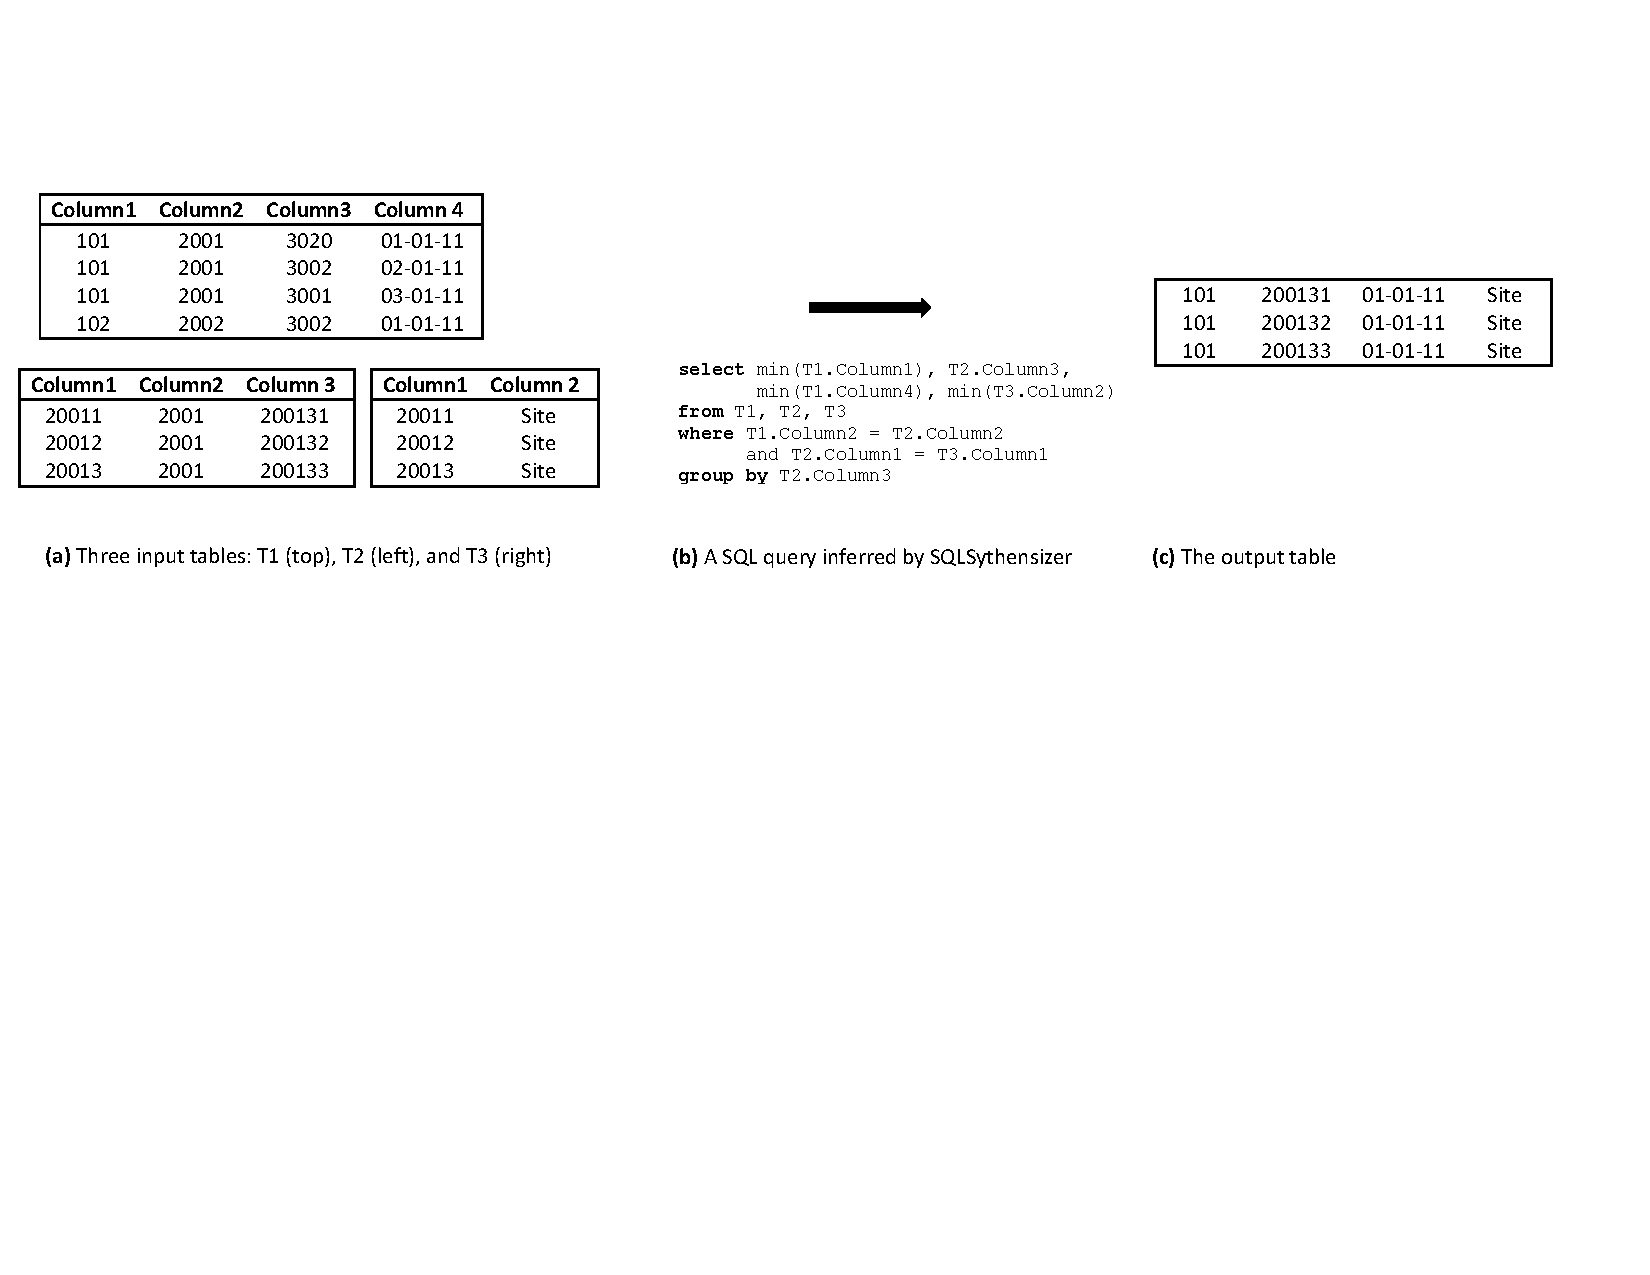
\includegraphics[scale=0.70]{example2}
  \vspace*{-1.0ex}\caption {{\label{fig:example2} Input-output
  examples ((a) and (c)) taken from an online SQL help forum
  thread. \ourtool automatically sythensizes 6 SQL queries that
  can produce the output table from the three input tables.
  (b) shows the highest ranked SQL query.
}}
\end{figure*}

We use a real SQL question from
an online forum\footnote{\url{http://forums.tutorialized.com/sql-basics-113/join-problem-147856.html}} to illustrate
\ourtool's effectiveness.
The question was started by a novice user, who needed help to write a
SQL query to get result from three input tables. In this question, the
novice user described his required query in a few paragraphs of
English, but also include several small, representative input-output
examples as shown in Figure~\ref{fig:example2}, to better express
his intention. 
This question receives no replies as of April 2013 and we speculated that
writing a SQL query to join three tables to produce certain output results
is non-trivial.

We ran \ourtool on the input-output examples
in Figure~\ref{fig:example2}. The tool produced 6 valid answers
in less than 1 minutes, all of which satisfy the given examples. The
highest ranked SQL query is shown in Figure~\ref{fig:example2},
which is quite unintuitive to write. The SQL query in
Figure~\ref{fig:example2}
first joins three input tables
on columns \CodeIn{T1.Column2}, \CodeIn{T2.Column2},
\CodeIn{T2.Column1}, and \CodeIn{T3.Column1} using some
selected columns, and then aggregates the results based on
column \CodeIn{Table2.Column3}'s value. Finally, it
returns the minimal values of columns \CodeIn{T1.Column1}, \CodeIn{T1.Column4}, and \CodeIn{T3.Column2}
from each aggregated group as the results.




\subsubsection{Performance}
\label{sec:performance}

We measured \ourtool�s performance by recording the average
time cost in producing a ranked list of SQL queries. 
As shown in Figure~\ref{tab:results}, the performance of \ourtool is
reasonable. On average, it uses less than \avgtime minutes to
produce the results in one interactive round.
Most of the time is spent querying the backend
database to validate the correctness of each synthesized  SQL query.
%\todo{caching might be helpful}



\subsubsection{Human Efforts}
\label{sec:human}

We measured the human efforts taken to use \ourtool in two ways.
First, the time cost to write input-output examples. Second,
the number of interactive rounds in invoking \ourtool
to synthesize the desirable SQL queries.

As shown in Figure~\ref{tab:results}, human efforts
spent in providing input-output examples are very limited:
on average, it took less than 5 minutes for one benchmark.
\todo{explain some abnormal points}

The number of interactive rounds is a measure of
the generalization power of the conditional learning part
of the algorithm and the ranking scheme.
We observed that the tool typically requires
just \avground rounds of interaction, when the user is smart
enough to give an example for each input format (which
typically range from 1 to 3) to start with. This was indeed the case
for most cases in our benchmarks, even though our algorithm
can function robustly without this assumption. The maximum number
of interactive rounds required in any scenario was \todo{XXX}
(with 2 to 3 being a more typical number). \todo{the largest table}
The maximum number of examples
required in any scenario over all possible interactions was 10.

\subsubsection{Comparison with an Existing Technique}.
\label{sec:comparison}

We compared \ourtool with \textit{Query By Output} (QBO), a
data-driven approach to infer SQL queries~\cite{Tran:2009}. We chose
QBO because it is the most recent technique and also one
of the most precise SQL query inference techniques in
the literature. QBO requires similar input as \ourtool, and
uses a decision-tree-based algorithm
\todo{explaining what is QBO}
However, QBO cannot infer SQL queries using \todo{aggregates}

The experimental results of QBO is shown in Figure~\ref{tab:results}
(Column ``Query by Example''). For all \exnum database exercises
and \pnum forum questions, QBO produces correct answers
for XXX and XXX of them, respectively. QBO fails to
synthesize desirable SQL queries for other benchmarks, because
it \todo{the reasons}.

We did not compared \ourtool with other related techniques~\cite{},
for three reasons. \todo{reasons}

\subsection{Experimental Discussion}

\noindent \textbf{\textit{Limitations.}}
The experiments indicate three limitations
of our technique. First, some query tasks
cannot be formulated by our SQL subset (Section~\ref{sec:langsubset})
due to unsupported features, such as
nested queries. This limitation is expected;
and our future work
should address this by including more SQL
features in \ourtool.
Second, on some examples, the learned query
conditions, though correct, are not precise
enough; and require users to provide more informative examples.
Take the example input and output in Figure~\ref{fig:rank}
as an example, \ourtool produces a SQL
query \CodeIn{select name from student where score > 2}
to satisfy the examples. However, if
the condition of the expected query
is \CodeIn{score > 3}, users must provide
one more tuple to the input table, such as "Chris, 3"
(a tuple with ``Chris'' in the name column and ``3''
in the score column), while keeping the output table
unchanged, 
to guide \ourtool to learn the correct query condition.
%Such imprecision is not caused by the limitation of
%\ourtool; rather, it reflects.
Third, \ourtool requires
users to provide noise-free input-output examples.
Even in the presence of a small amount of user-input
noises (e.g., a typo), \ourtool will declare failure
when it fails to infer a valid SQL query.
To overcome this limitation, we plan to design a more
robust inference algorithm that can attempt to identify
and tolerate user-input noises, and even suggest a fix
to the noisy example.

\vspace{1mm}
\noindent \textbf{\textit{Threats to Validity.}}
There are three major threats to validity
in our evaluation. First, the \exnum textbook exercises
and \pnum forum questions, though covering
a wide variety of SQL features, may not be representative enough.
Thus, we can not claim the results can be generalized to an
arbitrary use-case scenario. Second, we only compared
\ourtool with the \textit{Query by Output} technique~\cite{Tran:2009}.
Using other query inference or recommendation techniques
might achieve different results. Third, our
experiments focus on evaluating \ourtool's generality 
and accuracy. Even though all experiments are carried
out by a different person rather than \ourtool's developers,
it is unknown about \ourtool's general usability in practice.
To address this issue, we plan to conduct
a user study in our future work.


\vspace{1mm}
\noindent \textbf{\textit{Experimental Conclusions.}}
We have three chief findings: \textbf{(1)}
The supported SQL subset in \ourtool is
able to describe a variety of database queries.
\textbf{(2)} \ourtool can efficiently synthesize desirable SQL
queries with a small amount of human
efforts and small input-output examples.
\textbf{(3)} \ourtool produces better results
than an existing technique (\textit{Query by Output}~\cite{Tran:2009}).







\section{Related Work}
\label{sec:related}

We next discuss two categories
of related work on reverse engineering SQL queries 
and automated program synthesis.


%\subsection{Reverse Engineering SQL Queries}

\vspace{1mm}
\noindent{\textbf{\textit{Reverse Engineering SQL Queries.}}}
Reverse engineering SQL queries is a technique in the database
community~\cite{Zloof:1975, Tran:2009, DasSarma:2010} to
improve a database's usability. 
Zloof's pioneering work on \textit{Query by Example} (QBE)~\cite{Zloof:1975}
provided a high-level query language and a
form-based Graphical User Interface (GUI) for
writing database queries. To use the QBE system, 
users need to learn its query language,
formulate a query with the language, and fill in
the appropriate skeleton tables on the GUI.
By contrast, \ourtool mitigates such learning curves
by only requiring users to provide some representative
examples to describe their intentions

  %In other words, to derive a SQL query with the QBE system,
%end-users must learn a new query formulation language
%and explore its GUIs. These are the exactly
%two activities that may increase end-users' learning curve, and are avoided
%in \ourtool. \todo{exactly what we need to avoid.}



Tran et al.~\cite{Tran:2009} proposed a technique,
called \textit{Query by Output} (QBO), 
to find a set of semantically-equivalent SQL queries
to a given input query. QBO is related to but
significantly differs from \ourtool in two aspects.
First, QBO has a rather different goal and requires
slightly different inputs : it takes as inputs a database,
an SQL query, and the query's output (on the database); and computes
one or more equivalent queries that produce the
same output on the input database.
Second, QBO can only infer simple select-project-join queries,
while excluding many useful SQL features, such as aggregates,
the \CodeIn{HAVING} clause, and the \CodeIn{GROUP BY}
clause. As we demonstrated in Section~\ref{sec:evaluation},
QBO cannot infer queries for many use-case scenarios.
Its key limitation stems from the fact that it
only considers existing tuple values
in the input tables as features when learning
query conditions. 
By contrast, as shown in Section~\ref{sec:condition},
\ourtool addresses this limitation by enhancing
the existing tuple values with two kinds of
additional features, and thus is able to learn more
complex conditions.


Recently, Sarma et al.~\cite{DasSarma:2010} studied the \textit{View Definitions Problem} (VDP).
VDP aims to find the most
succinct and accurate view definition, when
the view query is restricted to a specific family of queries.
VDP can be solved as a special case in \ourtool where there is only one
input table and one output table. Furthermore, the main contribution
of Sarma et al's work is the complexity analysis of
three variants of the view definitions problem; there is no
tool implementation or empirical studies to evaluate
the proposed technique.

%Compared to \ourtool, there are three key differences:
%(1) VDP aims to infer a relation from a large representative
%example view, while \ourtool attempts to infer a SQL query from a
%set of few input-output examples \todo{revise below}
%(which is a critical usability aspect for end-users who lack adequate
%SQL experience). (2) the technique proposed by Sarma et al.~\cite{DasSarma:2010} does
%not consider join or projection
%operations and assumes the output view to be a strict subset of the input
%database with the same schema\todo{revise}, while our work eliminates these
%assumptions, and considers both join and projection operations.\todo{revise above}



%\todo{what is the limitation of non program sythesis, why
%sythensis would be useful.}

%\subsection{Automated Program Synthesis }

\vspace{1mm}

\noindent{\textbf{\textit{Automated Program Synthesis.}}}
Program synthesis~\cite{Gulwani:2010:DPS} is a useful
technique to create an executable program
in some underlying language from specifications that can range
from logical declarative specifications to examples or
demonstrations~\cite{Harris:2011, singh:2012, Gulwani:2011,
Kandel:2011, Fisher08Pads,Lau:2003:PDU, Lau:2000:VSA, Barbosa:2010:MLA, Arasu:2009:LST}.
It has been used recently for many applications.
%such as synthesis of efficient low-level code~\cite{Solar-Lezama:2005},
%data structure manipulations~\cite{Fisher:2008},
%geometry constructions~\cite{Gulwani:2011:SGC},
%snippets of excel macros~\cite{Harris:2011},
%relational data representations~\cite{Barbosa:2010:MLA, Arasu:2009:LST} and string
%expressions~\cite{singh:2012, Gulwani:2011}.


The PADS~\cite{Fisher:2008} system takes a large sample
of unstructured data and infers a
format that describes the data. Related,
the Wrangler tool, developed in the HCI community,
provides a visual interface for table transformations
and data cleaning~\cite{Kandel:2011}.
These two techniques, though well-suited for tasks
like text extraction, cannot be used to 
synthesize a database query.
This is because text extraction tasks
use completely different abstractions than a database query task,
and the existing tools like PADS and Wrangler lack the support for many database operations
such as joins and aggregation.

%text extraction tasks
%use completely different abstractions than a database query. and lack the support
%for many database operations like table joining, aggregations, etc.

%For example, while text extraction and mass editing
%are quite valuable for data transformation, the above tools
%lack other needed operations such as table joinning,
%aggregation, and query condition inference.
%\todo{explain}


Harris and Gulwani described a system for learning excel
spreadsheet transformation macros from an example
input-output pair~\cite{Harris:2011}. Given one input table and one output
table, their system can infer an excel macro that filters,
duplicates, and/or re-organizes table cells to generate the output table.
\ourtool differs in multiple respects.
First, excel macros have significantly different
semantics than the SQL language.
An excel macro can express a variety of table transformation operations
(e.g., table re-shaping), but are not capable to formulate database queries.
Second, Harris and Gulwani's approach treats table cells
as atomic units, and thus has different expressiveness
than \ourtool. For instance, their technique can generate macros to
transform one table to another, but cannot join multiple
tables or aggregate query results by certain table columns. 
%does not support queries
%involving conditions table joining, aggregation, or even column projection.
%\todo{examples}


%By contrast, \ourtool provides
%an interface based on examples, which is more
%friendly to end users. \todo{However, }


Some recent work proposed query recommendations systems
to enhance a database's usability~\cite{Howe:2011, Khoussainova:2010}. 
SQLShare~\cite{Howe:2011} is a web service that allows
users to upload their data and SQL queries,
%Each uploaded query is saved as a view, 
permitting other users
to compose and reuse. SnipSuggest~\cite{Khoussainova:2010} is a SQL autocompletion
system. As a user types a query, SnipSuggest mines existing query
logs to recommend relevant clauses or SQL snippets (e.g., the table
names for the \CodeIn{FROM} clause) based on the partial query that
the user has typed so far.
Compared to \ourtool, both SQLShare and SnipSuggest assume the
existence of a comprehensive query log
that contains valuable information.
%as a user articulates an increasingly larger fragment of a query.
However, such assumption often does not hold for
many database users in practice.
\ourtool eliminates this assumption and infers 
SQL queries using user-provided examples.


Cheung et al.~\cite{abs-1208-2013} presented a technique to infer SQL
queries from imperative code. Their technique transforms
fragments of application logic (written in an imperative language
like Java) into SQL queries. 
Compared to \ourtool, their work aims to help developers
improve a database application's performance,
rather than helping non-expert end-users
write correct SQL queries from scratch. 
If an end-user wishes to use their technique to 
synthesize a SQL query, she must write a snippet of
imperative code to describe the query task.
Comparing to providing example input
and output, writing correct imperative code is too challenging
for a typical end-user, and thus would
inevitably degrade the technique's usability.


%also cite this~\cite{Cheung:2012:UPS}, combining machine learning with program synthesis.


\section{Conclusions and Future Work}
\label{sec:conclusion}

Sai will write this section




\vspace{2mm}

%\noindent \textbf{Acknowledgement.} We would like
%to thank Stephen Fink and Manu Sridharan for
%answering our questions about WALA.
%\vspace{-2mm}

\bibliographystyle{abbrv}
\small{
\bibliography{sqlsynthesis}
}
\end{document}
